% Template for the submission to:
%   The Annals of Probability           [aop]
%   The Annals of Applied Probability   [aap]
%   The Annals of Statistics            [aos] 
%   The Annals of Applied Statistics    [aoas]
%   Stochastic Systems                  [ssy]
%
%Author: In this template, the places where you need to add information
%        (or delete line) are indicated by {???}.  Mostly the information
%        required is obvious, but some explanations are given in lines starting
%Author:
%All other lines should be ignored.  After editing, there should be
%no instances of ??? after this line.

% use option [preprint] to remove info line at bottom
% journal options: aop,aap,aos,aoas,ssy
% natbib option: authoryear
\documentclass[aoas]{imsart}

\newcommand{\ba}{ {\boldsymbol a} }
\newcommand{\bA}{ {\boldsymbol A} }
\newcommand{\bb}{ {\boldsymbol b} }
\newcommand{\bB}{ {\boldsymbol B} }
\newcommand{\bc}{ {\boldsymbol c} }
\newcommand{\bC}{ {\boldsymbol C} }
\newcommand{\bd}{ {\boldsymbol d} }
\newcommand{\bD}{ {\boldsymbol D} }
\newcommand{\be}{ {\boldsymbol e} }
\newcommand{\bE}{ {\boldsymbol E} }
\newcommand{\boldf}{ {\boldsymbol f} }
\newcommand{\bF}{ {\boldsymbol F} }
\newcommand{\bg}{ {\boldsymbol g} }
\newcommand{\bG}{ {\boldsymbol G} }
\newcommand{\bh}{ {\boldsymbol h} }
\newcommand{\bH}{ {\boldsymbol H} }
\newcommand{\bi}{ {\boldsymbol i} }
\newcommand{\bI}{ {\boldsymbol I} }
\newcommand{\bj}{ {\boldsymbol j} }
\newcommand{\bJ}{ {\boldsymbol J} }
\newcommand{\bk}{ {\boldsymbol k} }
\newcommand{\bK}{ {\boldsymbol K} }
\newcommand{\bl}{ {\boldsymbol l} }
\newcommand{\bL}{ {\boldsymbol L} }
\newcommand{\bm}{ {\boldsymbol m} }
\newcommand{\bM}{ {\boldsymbol M} }
\newcommand{\bn}{ {\boldsymbol n} }
\newcommand{\bN}{ {\boldsymbol N} }
\newcommand{\bo}{ {\boldsymbol o} }
\newcommand{\bO}{ {\boldsymbol O} }
\newcommand{\bp}{ {\boldsymbol p} }
\newcommand{\bP}{ {\boldsymbol P} }
\newcommand{\bq}{ {\boldsymbol q} }
\newcommand{\bQ}{ {\boldsymbol Q} }
\newcommand{\br}{ {\boldsymbol r} }
\newcommand{\bR}{ {\boldsymbol R} }
\newcommand{\bs}{ {\boldsymbol s} }
\newcommand{\bS}{ {\boldsymbol S} }
\newcommand{\bt}{ {\boldsymbol t} }
\newcommand{\bT}{ {\boldsymbol T} }
\newcommand{\bu}{ {\boldsymbol u} }
\newcommand{\bU}{ {\boldsymbol U} }
\newcommand{\bv}{ {\boldsymbol v} }
\newcommand{\bV}{ {\boldsymbol V} }
\newcommand{\bw}{ {\boldsymbol w} }
\newcommand{\bW}{ {\boldsymbol W} }
\newcommand{\bx}{ {\boldsymbol x} }
\newcommand{\bX}{ {\boldsymbol X} }
\newcommand{\by}{ {\boldsymbol y} }
\newcommand{\bY}{ {\boldsymbol Y} }
\newcommand{\bz}{ {\boldsymbol z} }
\newcommand{\bZ}{ {\boldsymbol Z} }
\newcommand{\vc}[1]{\mbox{\boldmath $#1$}}
\newcommand{\balph}{ {\boldsymbol \alpha} }
\newcommand{\balpha}{ {\boldsymbol \alpha} }
\newcommand{\bbet}{ {\boldsymbol \beta} }
\newcommand{\bbeta}{ {\boldsymbol \beta} }
\newcommand{\bgam}{ {\boldsymbol \gamma} }
\newcommand{\bgamma}{ {\boldsymbol \gamma} }
\newcommand{\bGamma}{ {\boldsymbol \Gamma} }
\newcommand{\bdelta}{ {\boldsymbol \delta} }
\newcommand{\bDelta}{ {\boldsymbol \Delta} }
\newcommand{\beps}{ {\boldsymbol \epsilon} }
\newcommand{\bepsilon}{ {\boldsymbol \epsilon} }
\newcommand{\bphi}{ {\boldsymbol \phi} }
\newcommand{\bPhi}{ {\boldsymbol \Phi} }
\newcommand{\bpi}{ {\boldsymbol \pi} }
\newcommand{\bpsi}{ {\boldsymbol \psi} }
\newcommand{\bkap}{ {\boldsymbol \kappa} }
\newcommand{\bkappa}{ {\boldsymbol \kappa} }
\newcommand{\bKappa}{ {\boldsymbol \Kappa} }
\newcommand{\blam}{ {\boldsymbol \lambda} }
\newcommand{\blambda}{ {\boldsymbol \lambda} }
\newcommand{\bLambda}{ {\boldsymbol \Lambda} }
\newcommand{\bmu}{ {\boldsymbol \mu} }
\newcommand{\bMu}{ {\boldsymbol \Mu} }
\newcommand{\bet}{ {\boldsymbol \eta} }
\newcommand{\bome}{ {\boldsymbol \omega} }
\newcommand{\bomega}{ {\boldsymbol \omega} }
\newcommand{\bOmega}{ {\boldsymbol \Omega} }
\newcommand{\bnabla}{ {\boldsymbol \nabla} }
\newcommand{\brho}{ {\boldsymbol \rho} }
\newcommand{\bsigma}{ {\boldsymbol \sigma} }
\newcommand{\bSig}{ {\boldsymbol \Sigma} }
\newcommand{\bSigma}{ {\boldsymbol \Sigma} }
\newcommand{\btheta}{ {\boldsymbol \theta} }
\newcommand{\bTheta}{ {\boldsymbol \Theta} }
\newcommand{\bzeta}{ {\boldsymbol \zeta} }
\newcommand{\bPsi}{ {\boldsymbol \Psi} }
\newcommand{\btau}{ {\boldsymbol \tau} }
\newcommand{\bxi}{ {\boldsymbol \xi} }
\newcommand{\bzero}{ {\boldsymbol 0} }
\newcommand{\bones}{ {\boldsymbol 1} }
\newcommand{\given}{\,|\,}
\newcommand{\sS}{{\cal S}}
\newcommand{\Ss}{{\cal S}}
\newcommand{\Field}{{\cal F}}
\newcommand{\colsp}{{\cal C}}
\newcommand{\nullsp}{{\cal N}}
\newcommand{\rowsp}{{\cal R}}
\newcommand{\tildeC}{\tilde{C}}
\newcommand{\tildeK}{\tilde{K}}
\newcommand{\tildew}{\tilde{w}}
\newcommand{\tildebw}{\tilde{\bw}}
\newcommand{\tildebW}{\tilde{\bW}}
\newcommand{\calC}{{\cal C}}
\newcommand{\calcbC}{{\bf {\cal C}}}

% Do not remove even for final version
\newcommand{\kcomment}[1]{{\color{blue}{\{KR: #1\}}}}
\newcommand{\kc}{\kcomment}


\usepackage{amsmath}
\usepackage{pstricks,pst-grad}
\usepackage{graphicx}
\usepackage{floatrow}
\usepackage[linesnumbered,ruled,vlined]{algorithm2e}
\floatsetup[table]{capposition=top}
% \usepackage{subfig}
\usepackage{subfigure}
\usepackage[utf8]{inputenc}

\usepackage[tableposition = top]{caption} % captions
\usepackage{booktabs}                     % horizontal lines in tables

% == Enable text degree
\usepackage{textcomp}

\usepackage{amsthm,amsmath,natbib}
\RequirePackage[colorlinks,citecolor=blue,urlcolor=blue]{hyperref}

% provide arXiv number if available:
%\arxiv{arXiv:0000.0000}

% == Trygve Test
\usepackage{color, colortbl}
\definecolor{Gray}{gray}{0.9}
\newcommand{\kcomment}[1]{{\color{red}{\{KR: #1\}}}}
\newcommand{\tofcomment}[1]{{\color{green}{\{TF: #1\}}}}
\newcommand{\kc}{\kcomment}
% put your definitions there:
\startlocaldefs
\endlocaldefs

\begin{document}

\begin{frontmatter}

% "Title of the paper"
\title{Informative Oceanographic Sampling using Excursion Probabilities for Multivariate Random Fields}
\runtitle{Excursion Probabilities for Informative Sampling}

% indicate corresponding author with \corref{}
% \author{\fnms{John} \snm{Smith}\corref{}\ead[label=e1]{smith@foo.com}\thanksref{t1}}
% \thankstext{t1}{Thanks to somebody} 
% \address{line 1\\ line 2\\ printead{e1}}
% \affiliation{Some University}

\author{\fnms{Trygve Olav} \snm{Fossum}\ead[label=e1]{trygve.o.fossum@ntnu.no}, \fnms{Jo} \snm{Eidsvik}\ead[label=e2]{jo.eidsvik@math.ntnu.no}, \fnms{David} \snm{Ginsbourger} \ead[label=e3]{david.ginsbourger@idiap.ch}  \and \fnms{Kanna} \snm{Rajan}\ead[label=e4]{kanna.rajan@ntnu.no}}

\address{Department of Marine Technology\\ Trondheim, Norway\printead{e1}}
\affiliation{Department of Marine Technology, The Norwegian University of Science and Technology (NTNU), Trondheim, Norway}

\address{Department of Mathematical Sciences \printead{e2}}
\affiliation{Department of Mathematical Sciences, NTNU}

\address{Idiap \printead{e3}}
\affiliation{Uncertainty Quantification and Optimal Design group, Idiap Research Institute, Martigny, Switzerland}

\address{Department of Engineering Cybernetics,\printead{e4}}
\affiliation{Department of Engineering Cybernetics, NTNU \&\\ Underwater Systems and Technology Laboratory, Faculty of Engineering, University of Porto, Portugal}

\runauthor{Fossum et al.}

\begin{abstract}
  Improving and optimizing oceanographic sampling is a crucial task for
  modern marine management and science faced with limited resources to
  understand highly dynamic processes in the water-column. The
  combination of statistics and autonomous
  robotics provides opportunities for studying aspects related to
  experimental designs for effective characterization of oceanographic
  phenomena. In this work we develop methods for efficient spatial
  sampling applied to the mapping of dynamic coastal processes by
  providing informative descriptions of spatial characteristics of ocean
  phenomena. Specifically, we define a design criterion based on
  reducing uncertainty in the excursion set of multivariate random
  fields, and derive analytical expressions for the expected Bernoulli
  variance reduction in the excursion set of spatial temperature and
  salinity variables. We show how these can be applicable in static
  designs and sequential designs, building on myopic and look-ahead
  sampling strategies. We use simulations to study the properties and
  differences between state-of-the-art approaches. Results from field
  deployments with an autonomous underwater vehicle are also presented,
  for a case study mapping the boundary of a river plume. The results
  demonstrate the ability of the method to effectively inform and
  execute data-driven environmental sampling.

%Motivated by the challenges related to efficient allocation of sampling resources in environmental sensing, the combination of Excursion Probabilities and Gaussian process modeling is explored for autonomous robotic sampling of ocean features; enabling information driven measures  sampling efforts to high-interest regions. These regions are usually characterized by gradients of measurable environmental variables, e.g., temperature or salinity gradients, on which EPs subsequently can be used...Correlation among samples and multivariate requirements are typical in environmental studies.
\end{abstract}

%\begin{keyword}[class=MSC]
%\kwd[Primary ]{}
%\kwd{}
%\kwd[; secondary ]{}
%\end{keyword}

\begin{keyword}
\kwd{Ocean Sampling}
\kwd{Excursion Sets}
\kwd{Gaussian Processes}
\kwd{Experimental design}
\kwd{Adaptive information gathering}
\end{keyword}

\end{frontmatter}

\section{Introduction}

Monitoring the worlds oceans has gained increased importance in the
light of the changing climate and increasing anthropogenic impact. A
central problem for understanding these factors is the lack of
representative data with sufficient resolution. Most of this
\emph{undersampling} can be attributed to the large spatio-temporal
variations on which ocean processes transpire, prompting the need for
effective means of sampling. By \emph{sampling}, we refer to the design
of observational strategies in the spatial domain, where the use of
autonomous platforms can be combined with statistical methods to pursue
measurements with high scientific relevance.

Traditional data collection at sea has typically been based on static
buoys, lagrangian floats or ship-based methods, with significant
logistical limitations that directly impact coverage and sampling
resolution. Modern methods using satellite remote-sensing provide
large-scale coverage, but have limited resolution, are limited to
sensing the surface of the ocean, and is impacted by cloud cover. The
advent of robust mobile robotic platforms \cite{Bellingham07} has
resulted in significant contributions to environmental monitoring and
sampling. In particular autonomous underwater vehicles (AUVs), have made
strides in advancing the state of sampling and consequently have made
robotics an integral part of ocean observation in large part by our own
work % driven by
% using statistical methods in design and data assimilation
\citep{das11b,Graham2013,Das2015,das15,fossuminformation,fossum18b}.
Others include \cite{wikle2013modern} focusing on hierarchical
statistical models, \cite{sahu2008space} which studies spatio-temporal
models for sea surface temperature and salinity data, while
\cite{mellucci2018oceanic} looks at the statistical prediction of
features using an underwater glider. Common to these approaches is the
use of information-based methods to infer environmental sampling. A few
important characteristics should be mentioned, namely:

\begin{itemize}
\item Decisions on where to sample happen sequentially, i.e.  how
  recently acquired information can be assimilated and used to improve
  statistical models and reduce uncertainty associated with where and
  when to make measurements.
\item As a priori information about the state of the ocean is very
  uncertain, there lies a substantial efficiency gain in reacting to
  information obtained from measurements taken \emph{in-situ}, this is
  usually referred to as the \emph{adaptivity gap} \citep{Krause2008phd}.
\item For such types of sampling problems, the number of choices (i.e.
  locations, trajectories, and candidate designs) makes the problem
  combinatorially large, creating a trade-off between optimization
  (finding the optimal design) and computability (arriving at a
  solution in reasonable time), which has to be considered in
  practice.
\end{itemize}{}

The combination of statistical tools and robotic platforms is a
natural symbiosis which enables information-based sensing. Central to
this is the ability to model spatially correlated variables and
provide formal measures of uncertainty. By far the most practical
models use Gaussian processes (GPs), which will also be used in our
formulation, in large part because it allows efficient implementation
and evaluation, in turn enabling prioritization of sampling efforts to
be formalized into decision making systems on-board a robotic
platform.

%Sampling can, in this context, not simply be distributed evenly ---along simple transects or ``lawn-mover" patterns--- but must instead be prioritized to relevant regions to ensure it is cost-effective while providing adequate coverage and resolution of the area of scientific interest.

%While the focus has often been on
%biological and anthropogenic impact from micro-plastics to
%pollution, biological oceanographers have focused intently on studying
%micro-organisms at the base of the human food web. These organisms are
%critically impacted by the changing dynamics in the upper water-column,
%especially in coastal zones which are complex and often hard to observe
%in space and time. By studying the bio-geochemical processes in the
%upper water-column scientists can measure the impact of change, natural
%or anthropomorphic, and provide an informed opinion to policy makers to
%effect changes in preserving the environment. However, the challenge of 
% The pressure on marine resources is growing and increased accuracy,
% resolution, and persistent monitoring of the oceans is crucial for
% long-term sustainable management. 

% A
% sustained focus on prioritized and efficient data collection strategies
% have therefore started to emerge. The advent of marine robotic
% platforms, especially

% provided means to execute this prioritization through the capacity of
% autonomy and data-driven sampling, where data collection in principle
% can be optimized. These capabilities have made

% of the emerging sensing practice for ocean science, allowing scientists
% to increase the observational efficiency and resolution beyond what was
% previously possible. But how should a robotic platform, such as an AUV,
% effectively prioritize and identify important regions for sampling? The
% answer to this question relates to 

% , and
% the application domain is clearly an arena where statisticians can
% contribute.
% There has recently been some statistical attention in oceanography:

%From an oceanographic perspective, interesting regions are usually directly tied to a distinct phenomena that is of scientific interest. Each phenomenon can in turn be characterized by a set of process specific conditions expressed through different measures of key environmental variables, such as temperature or salinity. One such measure is the gradient, that can be associated with a number of important processes, such as the vertical location of the thermocline and pycnocline, location of upwelling systems, vertical mixing, eddies, fronts, and currents \cite{sverdrup2006}, as well as distribution, growth, and accumulation of biological activity \cite{SatOceanSoci00, Ryan2014}. These gradients create boundaries separating the ocean into process specific regions which are of profound interest to both identify and map effectively. Quantification of gradient features is therefore a much needed competence in robotic sampling.

%The imperfect understanding of causality coupled with the underlying fundamental uncertainty of the ocean implies that we need to obtain more measurements and use statistical models and methods to determine what and how phenomena form, to increase the quality of predictive statements. 

In this work, we build on excursion sets (ES) and excursion
probabilities (EP) for spatial design of experiments. The goal is to
design sampling strategies for reducing the spatially integrated
Bernoulli variance (IBV) in the ES indicators.  The main contributions
involve: i) extending ES-based uncertainty criteria to multivariate
GPs, allowing the evaluation to include multiple environmental
parameters such as temperature and salinity, ii) developing methods
for informative environmental sensing and autonomous data collection,
and iii) demonstrating the approach in a real world scenario of
sampling a river plume using an AUV.

The remainder of the paper is organized as follows: Section
\ref{sec:bg} provides some background on ocean sampling. Section
\ref{sec:ESEP} defines ESs and EPs, and the design criteria of
IBV. Section \ref{sec:GP_EP} sets up the required statistical modeling
assumptions of the bi-variate GPs for temperature and
salinity. Section \ref{sec:sur} builds on these when deriving the
analytical derivation of the design criteria. Section
\ref{sec:heuristics} extends results to present heuristics for
adaptive sampling. Section \ref{sec:simulations} shows results and
discusses properties of the methods in simulation studies. Section
\ref{sec:case_study} demonstrates the methodology in field work
characterizing a river plume.  Section \ref{sec:concl_disc} contains
summary and a discussion of future work.


\section{Background and Motivation}\label{sec:bg}


\subsection{Observing Processes in the Upper Ocean}

% The processes occurring in the upper water-column and the photic zone
% (upper sunlit zone) are of vital importance for long-term sustainable
% management of the greater marine ecosystem, climate, and human health.
% With the onset of the warming oceans and increased anthropogenic
% pressure, it is critical to improve our understanding of the associated
% ecosystem response.

% owing to current observation practices.

Central to understanding the changes taking place in the upper
water-column is the understanding of biophysical interaction driven by
an agglomeration of physical forcing (wind, topography, bathymetry,
tidal influences and local geography such as fresh water inflows)
mixed with incipient micro-biology driven by planktonic and coastal
anthropogenic input, such as pollution and agricultural runoff. These
often result in a range of ecosystem related phenomena such as blooms,
anoxic zones and plumes, all with significant impact both directly and
indirectly on society. Walter Munk referred to the
20\textsuperscript{th} century as the \emph{century of undersampling}
\citep{munk2002}, pointing out that lack of sufficient sampling
resolution in time and space, as a critical issue for characterizing
ocean phenomena. Even today policy makers struggle with limited
observability of severe environmental problems such as the recent (May
2018) outbreak of harmful algal blooms in Northern
Norway\footnote{Report from the Institute of Marine
  Research:https://bit.ly/2KZGJfI}, with losses exceeding 12 million
tons of salmon valued at \$ 80 million (Norwegian Directorate of
Fisheries). This is a case in point in how adequate sampling efforts
could have provided a more accurate assessment and prior
warning. These challenges related to undersampling have been driving
ocean sensing practices towards more autonomous, networked and
distributed use of robotic assets in order to fill the gaps in our
understanding (See Fig. \ref{fig:envir}), where the surveying is
guided by a dynamical ocean model and the measurements made onboard
the robot are often used to update the model.

\begin{figure}[!h] 
  \centering 
  \subfigure[Illustration of an ocean sensing network, where robotic
  assets augment ship based measurements to increase coverage and
  resolution of phenomena of scientific interest.]{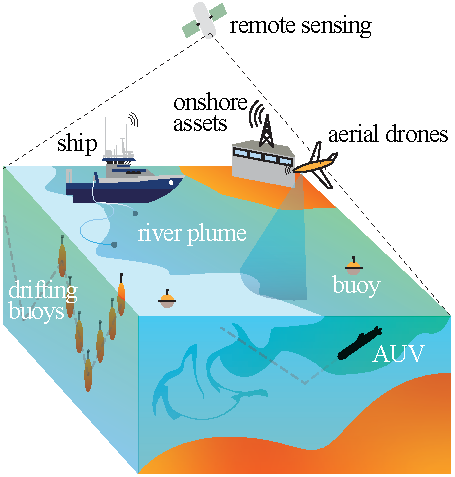
\includegraphics[width =
    0.48\textwidth]{Figures/envir.pdf}\label{fig:envir1}}
  \hfill
  \subfigure[Data-driven sampling under the sense-plan-act paradigm.]{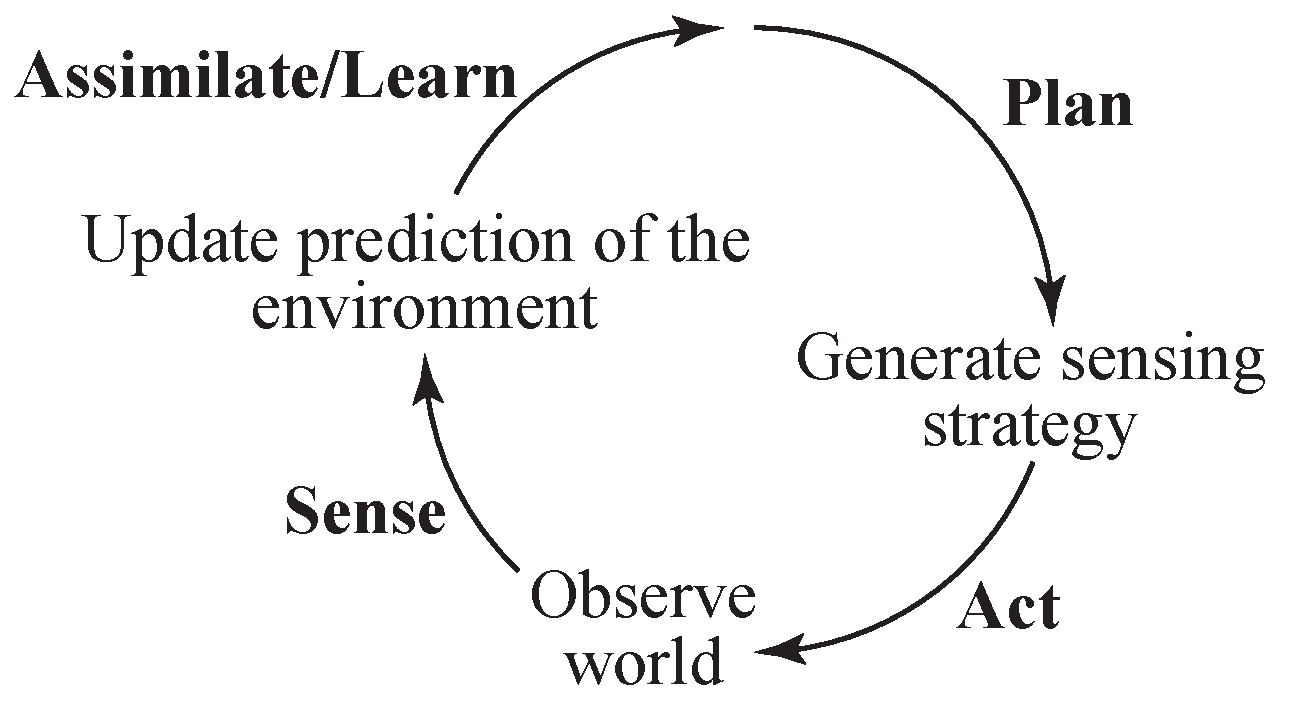
\includegraphics[width =
    0.48\textwidth]{Figures/adaptive_cycle.pdf}\label{fig:sense-plan-act}}
  \caption{Ocean observation is moving away from single-ship sampling
    towards more autonomous and collaborative networked operations in
    order to resolve the numerous bio-geochemical processes and their
    interactions.}
\label{fig:envir}
\end{figure}


Our focus in this work is towards spatial characterization of a
frontal system, and more specifically fronts generated by river
plumes. Fig. \ref{fig:nidelven} shows the survey area (the outlet of
the Nidelva river, Trondheim, Norway) where cold freshwater enters
from the river creating a strong gradient in both temperature and
salinity. Because of the local topography and the Coreolis force
\citep{coriolis1835memoire} the cold fresh water tends to flow near
land to the east. Depending on the river discharge, tidal effects,
wind and temperature differences, this boundary often gets
distorted. Prior knowledge about the location and evolution of these
features is therefore highly uncertain, making deterministic planning
challenging.

\begin{figure}[!h] 
\centering 
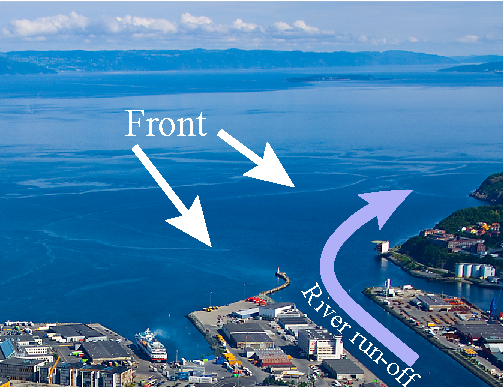
\includegraphics[width=0.85\textwidth]{Figures/pictures/c-updated.pdf}
\caption{Frontal patterns off of the Nidelva river, Trondheim, Norway.}
\label{fig:nidelven}
\end{figure}

%\begin{figure}[!h]
%\centering
 % \subfigure[River front - Columbia River, Astoria, Oregon, US.]{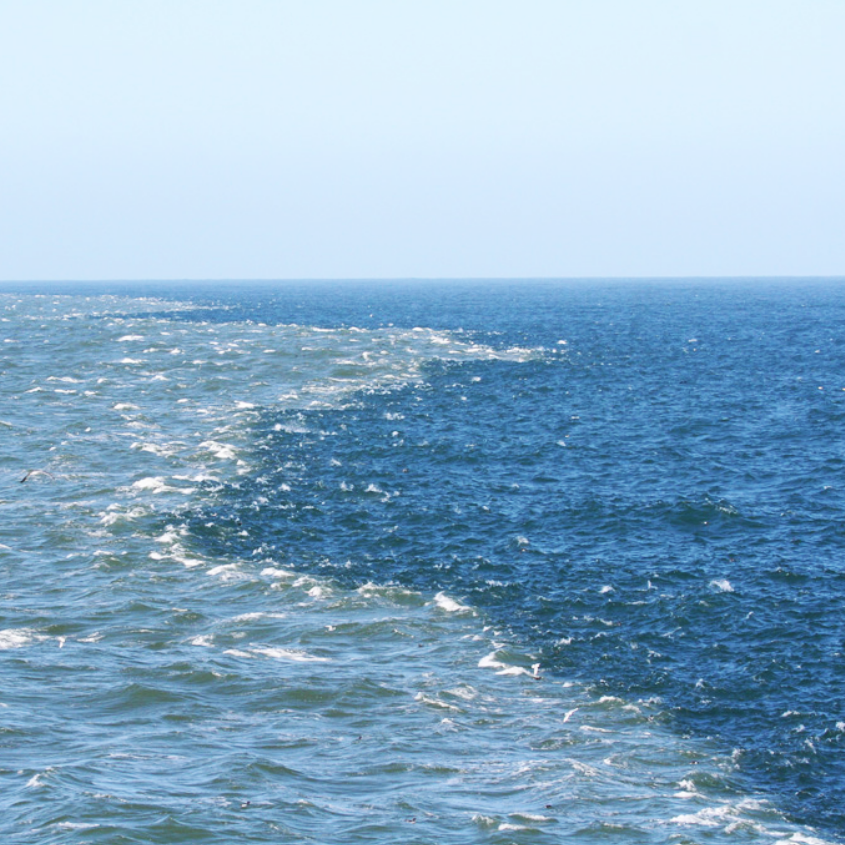
\includegraphics[width = 0.45\textwidth]{Figures/pictures/a.png}\label{fig:river1}}
 % \hfill
 %\subfigure[Tidal front - Korsfjorden, Norway.]{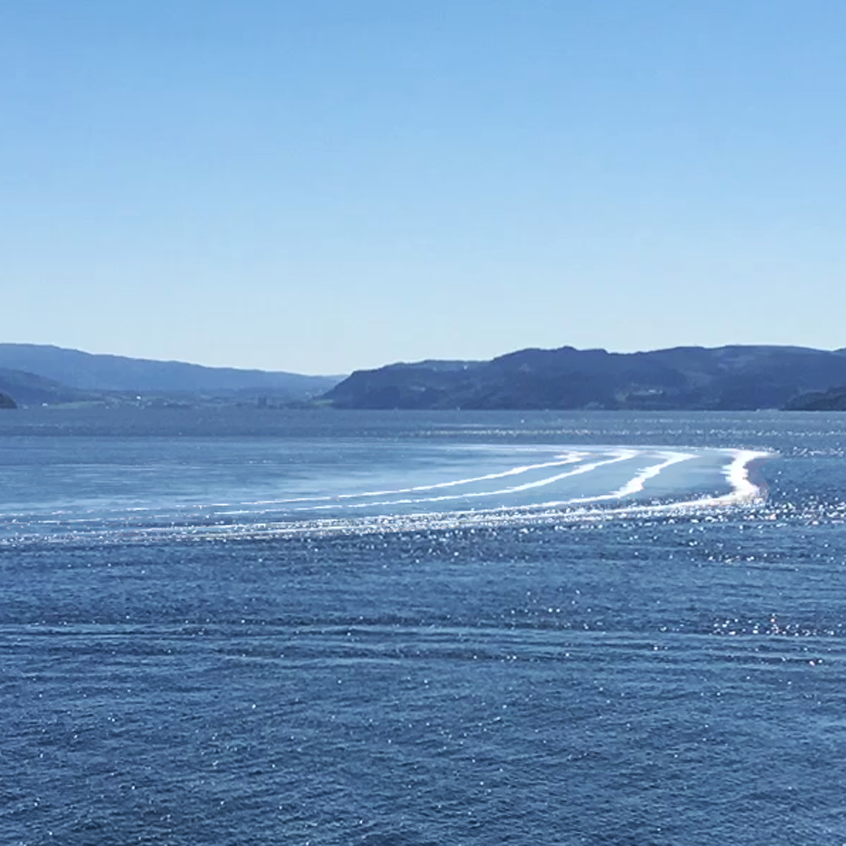
\includegraphics[width = 0.45\textwidth]{Figures/pictures/d.png}\label{fig:river2}}
 % \hfill
 % \subfigure[River plume - Rio de la Plata, Buenos Aires, Argentina.]{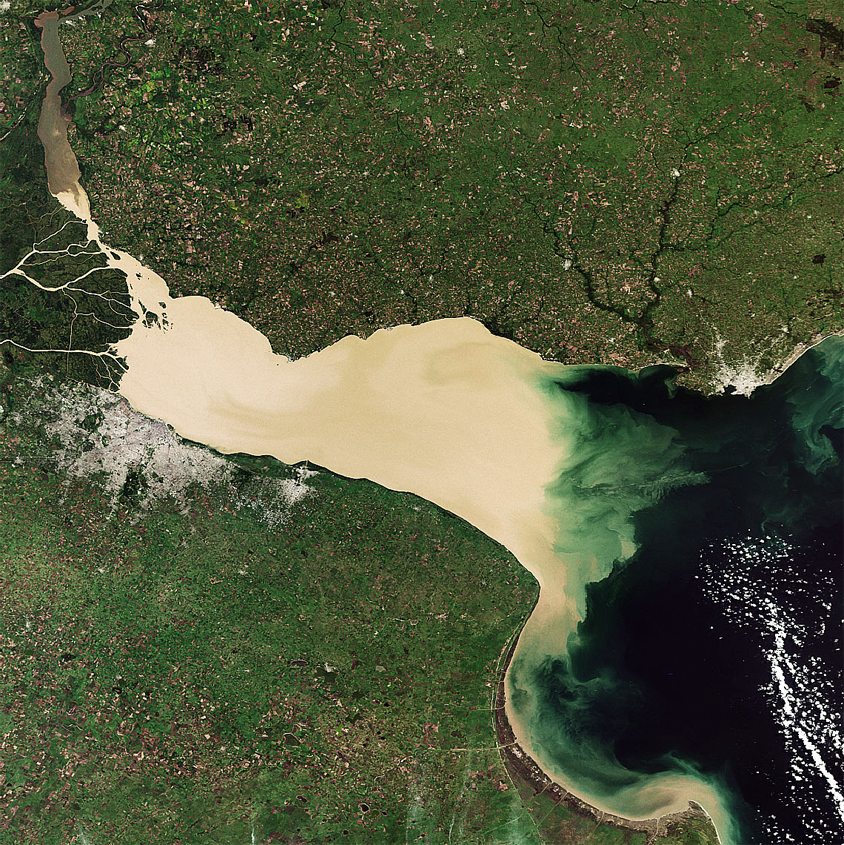
\includegraphics[width = 0.45\textwidth]{Figures/pictures/b.png}\label{fig:river3}}
 % \hfill
 %\subfigure[Frontal patterns - Nidelven, Trondheim, Norway.]{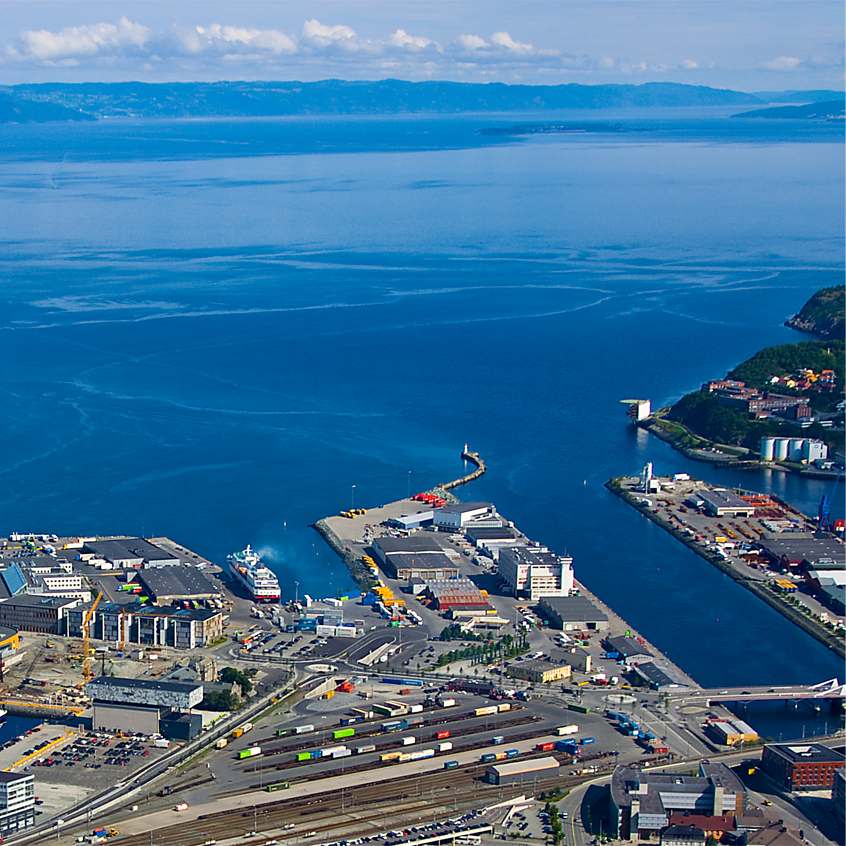
\includegraphics[width = 0.45\textwidth]{Figures/pictures/c.png}\label{fig:river4}}
 %\caption{Two examples of frontal features associated with
%   river-ocean interaction. % (\ref{fig:river1}) The river plume front of
   % the Columbia River meeting the Pacific Ocean.
%   (\ref{fig:river2})  Superimposed images (over 10 minutes) of a surface tidal front in
%   Korsfjorden, Norway. % (\ref{fig:river3}) The river plume of the Rio de
   % la Plata, taken by European Space Agency (ESA)'s Envisat platform and
   % MEdium Resolution Imaging Spectrometer (MERIS) sensor.
%   (\ref{fig:river4}) Aerial image of the mouth of the Nidelva river in
%   Trondheim, Norway where fresh water meets the salty fjord and creates
%   frontal patterns.} % Image courtesy: (\ref{fig:river1})
   % \cite{zamon2014marine}, (\ref{fig:river3}) ESA, CC BY-SA 3.0 IGO.}
% \label{fig:river_fronts}
%\end{figure}

%The use of \emph{robotic sampling} is motivated by the fundamental challenges of ocean observation, where a limited set of resources, a highly dynamic ocean, and the associated 

%This challenge can be addressed by employing more elaborate and adaptive sampling strategies that can capitalize on both prior and current observations in order to locate and map these areas.  

River plumes belong to a class of ocean processes that are local and
at smaller \emph{sub-mesoscale} (from $10 m^2$ -- $5 km^2$) where
spatial lateral variability tends to dominate. Remote sensing and
synthetic ocean models find it challenging to provide detail at this
scale \citep{Lermusiaux:2006} and the principal way to resolve for
fine resolution is by direct observation. At larger \emph{mesoscale}
($>50 km^2$), both three-dimensional space and time dynamics are
important and can shift substantially, while in the case of river
plumes one can often limit scope to cover only lateral spatial
elements. Moreover, for this case, time-effects can be regarded as
static when acquiring AUV data over a short time window and limited
region. However, the methodological framework can be extended to
higher dimensional situations in a similar manner.

\subsection{Autonomous Vehicles}

AUVs are used to gather in-situ spatio-temporal data from a targeted
domain while carrying a range of scientific payloads to survey the
water column.  Typically, they operate at $\sim 1-3$ m/s, can reach
depths from 100--6000m with an in-water staying capacity depending on
survey speed, payload sensors and mission design. By deploying AUVs
one can fill gaps in data gathering and augment information obtained
from either ocean models, remote-sensing data, or fixed-location
sensors on buoys. Traditional operations and surveys with AUVs are
usually limited to observations along fixed transects on a spatial
grid, pre-programmed by the human operator.  By using on-board
algorithms to continuously evaluate, update, and refine future
sampling locations, one can make information gathering adaptive and
contextual to the survey requirements
\citep{das11b,fossuminformation,fossum18b}. The space of sampling
opportunities is still limited to the spatial grid, but now there is
much more flexibility because of adaptation. For instance, an AUV
could reconstruct or modify a survey line based on what temperatures
it is measuring by using embedded methods in decision-theoretic
planning \citep{py10,Rajan12,Rajan12b}.

%To improve the state of sampling, modern tools and methods, including the use of autonomous platforms, oceanographic models and satellite remote sensing, needs to be combined with traditional data acquired by surface vessels or buoys (See Fig. \ref{fig:envir}). However, without adequate understanding of the theoretical underpinnings of how, when, and where to gather data, these tools and methods are insufficient in the vast and harsh oceans.

% retaining an advantageous strategy for information recovery, online during execution.
%The pressure on marine resources is growing and increased accuracy, resolution, and persistent monitoring of the oceans is crucial for long-term sustainable management. The impact of this research provides cost effective tools, techniques, and processes for doing ocean based measurements using robotic platforms. 
%adaptive design of experiments using robotic assets identifying and prioritizing relevant sampling locations on an information-theoretic basis. Spatial statistics naturally enters here through the ability to both model spatially correlated parameters and provide formal measures of uncertainty, on which this basis can be formed. 
%for oceanic sensing applications, where sensors are sparsely distributed and capitalizing on all available information is 

%This imperfect understanding of causality coupled with uncertainty implies that we need to obtain more measurements and use statistical models and methods to determine what and how phenomena form, to increase the quality of predictive statements. To improve the state of sampling, modern tools and methods, including the use of autonomous platforms, oceanographic models and satellite remote sensing, augment the more traditional data acquired by surface vessels or buoys (See Fig. \ref{fig:envir}). However, without adequate understanding of the theoretical underpinnings of how, when, and where to gather data, these tools and methods are insufficient in the vast and harsh oceans.

%There are several oceanographic data sources that can be used together with statistical tools to improve data collection in ocean science. In the following section we briefly discuss buoy data, satellite data, ocean models data, and AUV data.

%Buoy data provide very accurate information of oceanographic variables, but in most situations they are local, giving information only at one (north, east) coordinate, possibly with opportunities for conducting measurements at different depths. Gliders and other surface vessels are a kind of floating buoys that drift and can measure variables at many locations, but still with limited spatial coverage. 

%Satellite data are important for the mapping of oceanographic variables. They can also be indicative of variables such as temperature and salinity which we look at here, especially if the data are calibrated to for instance buoy data from the same spatial domain. However, the resolution of satellite data is relatively large, say $1 \times 1$ km $^2$ grid cells, and it only provides accurate information at the sea surface. Moreover, one cannot get useful satellite information on a cloudy day. 

%What is often done in practice is to run ocean models based on the complex differential equations governing oceanographic phenomena, where also satellite data can be assimilated and used as input, and possibly playing with different forcing mechanisms to capture some of the uncertainty of the models. Initial conditions, and can be used t the goal is to guide the sampling towards regions these regions, where we can reduce the uncertainty in the ES. These models provide insight that can be understood from practitioners, but they tend to be biased, and must also be calibrated to buoy data in one way or the other.

%to provide an effective specification of regions of phenomenological interest resolving the boundaries and the position of phenomena, on which evaluation of future sampling can be constructed.

%; some of these phenomena are illustrated in Fig. \ref{fig:envir2}. Figure \ref{fig:river_fronts} illustrates the %phenomena of interest in this paper, which is river plumes and their interaction with the ocean.

%Feature driven sampling
%processes acting across a wide range of spatio-temporal scales makes prioritizing sampling efforts necessary. %Autonomous robotic platforms, can address these issues by providing the ability to focus sampling efforts to %high-interest regions (``hotspots").


% Determining paths for mobile robotic sensors in order to maximize the
% information gained about an environment is formally known as informative
% path planning. This, and related problems such as the orienteering
% problem \citep{Golden87}, has been studied in the context of graphs,
% where the potential measurement are assigned to nodes on which
% evaluation of different routes can be conducted.
%In this context, a fundamental result from \cite{nemhauser1978analysis} proves that a simple greedy algorithm (iteratively selecting the location which most increases the utility) can achieve a near-optimal solution if the problem can be shown to be \emph{submodular}\footnote{an intuitive diminishing returns property, where the informative value of adding sensors decrease with the number of sensors added.}. Building on this result, \cite{chekuri2005recursive} explored this in the setting of a graph using a recursive greedy algorithm, providing near-optimal solutions depending on the planning horizon and graph resolution. 

Adaptive sampling of an evolving frontal feature has been explored in
\cite{fronts11,Zhang2012,Pinto2018,costa19}. These approaches
typically use a reactive-adaptive scheme, whereby exploration does not
rely on a statistical model of the environment, but rather adapts
based on closing the sensing and actuation loop
(Fig. \ref{fig:sense-plan-act}). Myopic sampling, i.e. step-wise
selection of the path (on the graph) which reduces the information
criterion the most, has been used for adaptive surveys
\citep{singh2009efficient,Binney2013} which focus largely on reducing
predictive variance or mutual information (entropy). Variance and
entropy reduction are independent of the actual data realizations
under the assumption of GP models, and the use of data-driven adaptive
criteria was introduced to include more targeted sampling of regions
of scientific interest by \cite{Low2009} and \cite{fossuminformation}.
In this paper, with the focus on mapping the river plume, we reward
the designs that improve the classification of water masses, as a
means to characterize the frontal zone.

%\begin{figure}[h]
%\centering
%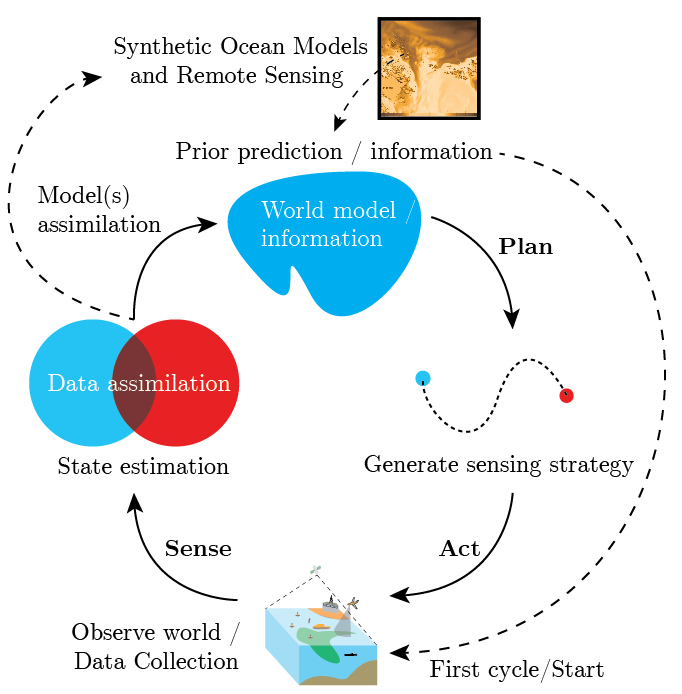
\includegraphics[width=0.4\textwidth]{Data-driven.png}
%\label{fig:auv_alone}
%\caption{The concept of data-driven sampling.}
%\end{figure}

%The goal is effectively map the extension of the river plume given this


%, we can formulate this question as follows: the ocean region  defined by the boundary between water bodies, separated by a characteristic temperature gradient that is smaller than $T=5$\textdegree C and a salinity concentration lower than $S=30$ [g/kg]. A goal is then to improve our predictive capabilities to answer this question better.
%For example,  (examples are shown in Fig. \ref{fig:river_fronts}). However, 

% In doing so, the aim is to increase the knowledge about the uncertain ocean environment through adaptive sampling


\section{Excursion sets and Integrated Bernoulli variance}
\label{sec:ESEP}

Our objective is to characterize a river plume, focusing on spatial
separation of cold freshwater from the warmer saline waters of the
fjord. Excursion sets (ES) and excursion probabilities (EP) are useful
starting points to measure the ability to classify water masses. The
goal of experimental sampling is to improve this characterization, as
quantified via changes in the EPs.

We consider a lateral domain, near the sea surface, with locations
$\bx \in \mathcal{M} \subset \mathbf{R^2}$. The two variables of
interest, temperature and salinity, are defined as random processes;
$\xi_a(\bx)$ denotes the temperature (in $^o C$) and $\xi_b(\bx)$
denotes the salinity (in $mg/l$) at location $\bx$. \kc{might be
  clearer if you used 't' for temp and 's' for salinity. 'a' and 'b'
  are somewhat opaque especially further in the text. Also there
  should be a statement about why we're considering only 2 variables
  and the impact to considering (algebraically) more in the following
  formulations. This will surely be asked by any reviewer.}.  We let $t_a$ be a
threshold for temperature and $t_b$ a threshold for salinity, the
bivariate ES is then defined by:

\begin{equation}\label{ES}
     \mbox{ES} = \{\bx \in \mathcal{M} | \xi_a(\bx) \leq t_a,\xi_b(\bx) \leq t_b\}.
\end{equation}
The excursions could also be defined as larger than a threshold, or
within a boundary of limits for the two variables; calculations and
interpretations will be similar in these cases.

The ES holds random indicator variables, while the associated EPs are: 
\begin{equation}\label{eq:prob}
  p(\bx) = P(\xi_a(\bx) \leq t_a, \xi_b(\bx) \leq t_b), \hspace{3mm} \bx \in \mathcal{M}.
\end{equation}
If the EPs in Eq. (\ref{eq:prob}) are
close to $1$ or $0$, it is easy to classify water masses; it is
challenging if the probabilities are close to $0.5$. 
The integrated Bernoulli variance (IBV) \cite{bect2019}, is defined as: 
\begin{equation}\label{measVAR}
    V = \int_{\bx \in \mathcal{M}} p(\bx) \left(1-p(\bx)\right) d\bx.
\end{equation}
The measure is dominated by locations with EPs close to $0.5$.
\kc{This sentence is a bit strange; just about, you state that EPs
  close to 0.5 can be problematic since they do not categorize the
  water masses well. And here you state that there is a strong
  dominance of the average. So now you should say how the biasing can
  change to make ``V'' more effective. Otherwise this sentence is
  dangling.} 

If prior knowledge provides a strong indication of cold freshwater
(for instance) in a part of the domain, it is easy to classify, and
there is likely little value in exploring those locations. Data can be
gathered at selected locations of the domain $\mathcal{M}$, to improve
classification skill. We denote temperature measurements by
$y_{a}(\bx_i)$ and salinity measurements by $y_{b}(\bx_i)$, at a
sampling location $\bx_i \in \mathcal{M}$. Given a set of
measurements, denoted $\by$, the conditional EPs are:
\begin{equation}\label{eq:post_ep}
 p(\bx;\by) = P(\xi_a(\bx) \leq t_a, \xi_b(\bx) \leq t_b |\by). 
\end{equation}

Our goal is to construct designs for data gathering, that are expected
to improve the mapping and separation of water masses. When designing
AUV sampling designs, it is therefore natural to evaluate the expected
reduction in the IBV, as provided by the survey data. In this way, we
take the expectation with respect to the planned measurements $\by$;
\begin{equation}\label{sur}
    V_{\mbox{upd}} = \int_{\bx \in \mathcal{M}} E_{\by} \left\{ p(\bx;\by)\left( 1-p(\bx;\by)\right) \right\} d\bx, 
\end{equation}
where the probability is defined in Eq. (\ref{eq:post_ep}).
Considering a set $\mathcal{J}$ of possible designs for an AUV survey. A criterion for the selection is:
\begin{equation}\label{crit}
    j^* = \mbox{argmin}_{j \in \mathcal{J}} V_{\mbox{upd}}(j),
\end{equation}
where the criterion $V_{\mbox{upd}}(j)$ in Eq. (\ref{sur}) is computed
for each of the possible designs. 

Recent work on ESs and EPs connected to spatial statistics include
\cite{picheny2010,french2013spatio,bolin2015excursion,french2016credible}.
Our focus is on ES as defined in Eq. (\ref{ES}), and the uncertainty
reduction achieved by sampling as in Eq. (\ref{sur}). In this sense
our work is similar to \cite{bect2012}, \cite{chevalier2014fast} and
\cite{azzimonti2016quantifying} who describe analytical results for
uncertainty reduction in ESs for univariate processes. A major
contribution of our work is to derive closed-form results for this
design criteria in the situation with multivariate GPs.

\section{Gaussian processes and excursion probabilities}
\label{sec:GP_EP}

Calculations of the EPs and the IBV require a model specification.
Here, we use Gaussian modeling assumptions which allow closed form
evaluation of the IBVs, as derived in Section \ref{sec:sur}.

\subsection{Bivariate Gaussian processes}

We represent the bivariate random fields of temperature and salinity
with a Gaussian model. At location $\bx \in \mathcal{M}$, the
bivariate distribution is:
\begin{equation}\label{gp_bar}
  \begin{bmatrix}\xi_a(\bx) \\
    \xi_b(\bx) \end{bmatrix}
 \sim N \left( 
\begin{bmatrix} \mu_{a}(\bx)\\
\mu_{b}(\bx)
\end{bmatrix},\begin{bmatrix}
\sigma_{a}^2(\bx) & \sigma_{a}(\bx) \sigma_b(\bx) \gamma(\bx)  \\
\sigma_{a}(\bx) \sigma_b(\bx) \gamma(\bx)  & \sigma_{b}^2(\bx) 
\end{bmatrix}
\right),
\end{equation}
where the notation refers to Gaussian (Normal) distributed variables
specified by the mean vector and covariance matrix. In the application
below, the model parameters are specified from preliminary data: The
mean varies with location, capturing the variability near the river
mouth, while the variance parameters and correlation between salinity
and temperature are assumed to be constant for all locations. \kc{?
  Isn't that too strong an assumption? T/S tend to be correlated,
  however for uniform bodies of water; here we're dealing with coastal
  ecosystems where the two are not necessarily so.}

For the spatial dependence among variables, 
we assume a separable correlation function with the same decay for salinity and temperature,
which is not unrealistic for a river plume \kc{why so?}. We have:
\begin{equation}\label{gp_corr}
\mbox{Cov}(\xi_i(\bx),\xi_j(\bx')) = \rho(\bx,\bx') \sigma_i \sigma_j (\gamma +(1-\gamma )\delta_{ij}), \\
\end{equation}
for $i,j \in {a,b}$ and $\delta_{ij}=1$ if $i=j$ and $\delta_{ij}=0$
otherwise. Moreover, we assume a stationary isotropic property
\kc{This is probably related to the assumption as above where T/S are
  assumed to be constant in all locations? But why?} where the
correlation function $\rho(\bx,\bx')$ solely depends on $\bx$ and
$\bx'$ via a Euclidean distance measure $h=\sqrt{|\bx-\bx'|^2}$. With
data and prior knowledge one could possibly fit and estimate
parameters of non-stationary or non-isotropic covariance functions and
more complex multivariate spatial covariance functions
\citep{gneiting2010matern,genton2015cross}; however that is left for
future work.

For implementation purposes, we discretize the spatial domain
$\mathcal{M}$ to a set of $n$ grid locations
$\mathcal{M}_g = \{\bx_i, i=1,\ldots,n \}$, where each cell has area
$\Delta$. The integral expression in Eq. (\ref{measVAR}) and
(\ref{sur}) are then approximated by sums over all grid cells. This
grid is identical to the possible set of design locations and defined
as a waypoint graph \kc{You mean the
  centroids of the cells are part of the graph?}. Using vector
notation, we denote the Gaussian temperature and salinity variables on
the grid and its density function by: 
\begin{equation}\label{prior}
    \bxi = (\xi_a(\bx_1),\xi_b(\bx_1),\ldots,\xi_a(\bx_n),\xi_b(\bx_n))^t, \hspace{3mm}
    \bxi  \sim  N(\bmu, \bSigma) %\pi (\bxi) & =& \frac{1}{(2\pi)^{n}|\bSigma|^{\frac{1}{2}}}e^{-\frac{1}{2}(\bxi -\bmu)^T\bSigma^{-1}(\bxi-\bmu)}.
\end{equation}
%Here, $\pi(\bxi)$ is the joint density function of length $2 n$ vector $\bxi$, and
The length $2 n$ vector $\bmu$ holds the expected values of
temperature and salinity at the grid locations, while the
$2n \times 2n$ positive definite matrix $\bSigma$ holds the
variance-covariances of temperature and salinity variables at all grid
locations.

\subsection{Data model and updating of Gaussian processes}

Data is gathered by an AUV that can measure temperature and salinity
at a subset of locations on the defined grid. This can be done in a
static manner, where the survey design is pre-planned, or in a
sequential way with several rounds of data gathering. For the latter,
a round of data is gathered first, and then assimilated to get an
updated model. Then the updated model is used to design and select the
next round of measurements, and so on. We describe the model for one
round of data and the Gaussian formula for a single update. In Section
\ref{sec:heuristics} we discuss sequential data gathering in the
context of adaptive design of AUV measurements.

We denote the data at $n_y$ locations by
$\by=(y_{a,1},y_{b,1},\ldots,y_{a,n_y},y_{b,n_y})^t$, representing the
temperature and salinity measurements gathered at the first round of
nodes in the grid. The conditional model for the data, given the true temperature
and salinity, is described by: 
\begin{equation}\label{likelihood}
\by | \bxi \sim N( \bA \bxi, \bR), %\pi(\by | \bxi)= \frac{1}{(2\pi)^{m}|\bR|^{\frac{1}{2}}}e^{-\frac{1}{2}(\by -\bA\bxi)^T\bR^{-1}(\by-\bA\bxi)},
\end{equation}
where $\bA$ is an $2n_y \times 2n$ matrix holding '$1$'s on the
measurement indices on the grid and '$0$' otherwise. The size
$2n_y \times 2n_y$ covariance matrix $\bR$ contains diagonal entries
$r^2_a$ and $r^2_b$ which are measurement error variances of
temperature and salinity observations.

The GP mean and covariance in Eq. (\ref{prior}) are moderated \kc{What
  does 'moderated' mean?} when more information is available. The
updated distribution for temperature and salinity variables on the
spatial grid, given survey data $\by$, is Gaussian with mean and
covariance: 
\begin{eqnarray}\label{gp_upd}
  \bm &=& \bm(\by) = \bmu+\bSigma \bA^t (\bA \Sigma \bA^t+\bR)^{-1}(\by-\bA \bmu),  \\
  \bS &=& \bSigma - \bSigma \bA^t (\bA \bSigma \bA^t+\bR)^{-1} \bA
          \bSigma.\nonumber
\end{eqnarray}

The updated bivariate distribution at a grid location $\bx \in
\mathcal{M}_g$ is then: 
\begin{equation}\label{gp_hat}
\begin{bmatrix}
\xi_a(\bx) \\
\xi_b(\bx)
\end{bmatrix}
 |\by
 \sim N \left( 
\begin{bmatrix} m_{a}(\bx)\\
m_{b}(\bx)
\end{bmatrix},\begin{bmatrix}
s_{a}^2(\bx) & s_{a,b}(\bx)  \\
s_{a,b}(\bx)  & s_{b}^2(\bx)  
\end{bmatrix}
\right),
\end{equation}
with entries extracted from the conditional mean and covariance
expressions in Eq. (\ref{gp_upd}).

% The conditional mean $\bm$ will be important in the following
% derivation in Section \ref{sec:sur}.
The calculation of the design criterion in Eq. (\ref{sur}) requires
the marginal distribution of the data which is defined over $\bxi$ to
be $\by \sim N( \bA \bmu,\bA \bSigma \bA^t+\bR)$.  However, it turns
out that a simplified form of the calculation is possible because the
conditional mean in Eq (\ref{gp_hat}) is a linear (affine) function of
the data $\by$ and the covariance is not a function of the data.
Before knowing the data, the distribution of the conditional mean is
\begin{equation}\label{distxi} \bm \sim N(\bmu , \bPsi), \hspace{3mm}
  \bPsi=\bSigma \bA^t (\bA \bSigma \bA^t+\bR)^{-1} \bA \bSigma.
\end{equation} 
When considering only grid location $\bx$, we can
extract elements from its mean vector and covariance matrix to get the
bivariate distribution \begin{equation}\label{dist_mxi} 
  \bm(\bx) \sim N \left( \begin{bmatrix}
      \mu_{a}(\bx) \\
      \mu_{b}(\bx) \end{bmatrix}, \begin{bmatrix}
      \psi^2_{a}(\bx) & \psi_{a,b}(\bx)\\
      \psi_{a,b}(\bx) & \psi^2_{b}(\bx) \end{bmatrix} \right),
\end{equation}
which is important for the derivation of the closed form solution of the design criteria.

\section{Uncertainty reduction in excursion sets}
\label{sec:sur}

\subsection{Excursion probabilities for Gaussian processes}

Based on Gaussian modeling assumptions, the EPs can be computed at any
location $\bx$. Without additional data, Eq.  (\ref{eq:prob}) gives us:

\begin{eqnarray}\label{eq:prob_mv0}
 p(\bx) &=& P(\xi_a(\bx) \leq t_a, \xi_b(\bx) \leq t_b) \nonumber \\
 &=& \Phi_2 \begin{pmatrix} 
\begin{bmatrix} t_a\\
t_b
\end{bmatrix};
\begin{bmatrix} \mu_{a}(\bx)\\
\mu_{b}(\bx)
\end{bmatrix},\begin{bmatrix}
\sigma_{a}^2(\bx) & \sigma_{a}(\bx)\sigma_{b}(\bx) \gamma(\bx)  \\
\sigma_{a}(\bx)\sigma_{b}(\bx) \gamma(\bx)  & \sigma_{b}^2(\bx)  
\end{bmatrix}\end{pmatrix},
\end{eqnarray}
where $\Phi_2$ is the bivariate Gaussian cumulative distribution
function, and the mean and covariance entries are as defined in Eq. (\ref{gp_bar}).

When data $\by$ are available, Eq. (\ref{eq:post_ep}) similarly gives
us:
\begin{eqnarray}\label{eq:prob_mv}
 p(\bx;\by) &=& P(\xi_a(\bx) \leq t_a, \xi_b(\bx) \leq t_b |\by)
 \nonumber \\
 &=& \Phi_2 \begin{pmatrix} 
\begin{bmatrix} t_a\\
t_b
\end{bmatrix};
\begin{bmatrix} m_{a}(\bx)\\
m_{b}(\bx)
\end{bmatrix},\begin{bmatrix}
s_{a}^2(\bx) & s_{a,b}(\bx)  \\
s_{a,b}(\bx)  & s_{b}^2(\bx)  
\end{bmatrix}\end{pmatrix},
\end{eqnarray}
with parameters as defined in Eq. (\ref{gp_upd}) and (\ref{gp_hat}).

\subsection{Expected Integrated Bernoulli variance for bivariate models}

We will next derive closed form solutions to the expectation in
(\ref{sur}). The location index $\bx$ is suppressed to avoid overly
complex notation. We present new results for computing the expectation
$E_{\by}\left\{ \cdot \right\}$ which is the integrand of
Eq. (\ref{sur}).

A critical first element in the derivation is the GP model, and the
linear dependence on $\by$ in the conditional mean in
Eq. (\ref{gp_upd}), which results in a closed form Gaussian
distribution for the conditional mean in Eq. (\ref{dist_mxi}). The
high-dimensional inner integral in Eq. (\ref{sur}) then reduces to a
bivariate integral \citep{bhattacharjya2013value, chevalier2014fast},
with expectation over $\bm=(m_{a},m_{b})^t$.  We standardize the two
variables in Eq. (\ref{sur}), i.e.  $Z_a=\frac{\xi_a-m_{a}}{s_{a}}$,
$Z_b=\frac{\xi_b-m_{b}}{s_{b}}$, and then
\begin{eqnarray}\label{ytom}
   P(\xi_a \leq t_a, \xi_b \leq t_b|\by) &=& P \left( Z_a \leq\frac{t_a-m_{a}}{s_{a}}, Z_b \leq\frac{t_b-m_{b}}{s_{b}}|\by \right) \nonumber \\
   &=& \Phi_2 \begin{pmatrix} 
\begin{bmatrix} \frac{t_a-m_{a}}{s_{a}}\\
\frac{t_b-m_{b}}{s_{b}}
\end{bmatrix};
 \begin{bmatrix} 0\\
0
\end{bmatrix},\begin{bmatrix}
1 & \eta_{s,t}  \\
\eta_{s,t}   & 1  
\end{bmatrix}\end{pmatrix} \nonumber \\
&=& P(\xi_a \leq t_a, \xi_b \leq t_b|\bm),
\end{eqnarray}
where $\eta_{a,b} =s_{a,b}/(s_{a} s_{b})$.
%Since the expression only depends on $\by$ via $\bm$, the expectation in Eq. (\ref{sur}) is reduced to a bivariate integral over $\bm$ (which will vary for each integrand term, because the locations differ). 

Using Eq. (\ref{ytom}) and introducing $\pi(\bm)$ for the density
function of $\bm$, the expected Bernoulli variance becomes:
\begin{eqnarray}\label{eq:var2}
E_{\by}(p(1-p)) &=& E_{\bm}(p(1-p)), \hspace{3mm} p=P(\xi_a \leq t_a, \xi_b \leq t_b|\bm) \nonumber \\
E_{\bm}(p(1-p)) & = & \int p[1-p] \pi(\bm) d\bm, \nonumber \\
 &=& \int P(\xi_a \leq t_a, \xi_b \leq t_b|\bm)  \pi(\bm) d\bm \nonumber  \\
&-& \int P(\xi_a \leq t_a, \xi_b \leq t_b|\bm) P(\xi_a \leq t_a, \xi_b \leq t_b|\bm) \pi(\bm) d\bm. 
\end{eqnarray}
We will next extend results of \cite{chevalier2014fast} to solve for
these two parts (see also \cite{stroh} for such an extensions).

For the first part of the above, we have:
\begin{equation}\label{part1:phi2}
 \int P(\xi_a \leq t_a, \xi_b \leq t_b|\bm) \pi(\bm) d\bm= 
P \left( Z_{a} \leq \frac{t_a-m_{a}}{s_{a}}, 
Z_{b} \leq \frac{t_b-m_{b}}{s_{b}} \right), \nonumber
\end{equation}
where $\bZ=(Z_{a},Z_{b})$ is a bivariate zero-mean and unit-variance
Gaussian vector, with $\mbox{Corr}(Z_{a},Z_{b})=\eta_{a,b}$. Moreover,
$\bZ$ is chosen to be independent of $\bm$. Using Eq. (\ref{dist_mxi})
we have
\begin{equation}
    E(s_{a} Z_{a}+m_{a}-t_a) = \mu_{a}-t_a, \hspace{3mm}
    \mbox{Var}(s_{a} Z_{a}+m_{a}-t_a) = s^2_a+ \psi^2_{a}, 
\end{equation}
and the same holds for the salinity part with subscript $b$ \kc{I
  really think this 'a' 'b' business should go and be more descriptive
  or intuitive.}. From this we get:
\begin{eqnarray}\label{two_parts0}
& P & \left( Z_{a} \leq \frac{t_a-m_{a}}{s_{a}}, 
Z_{b} \leq \frac{t_b-m_{b}}{s_{b}} \right) \\
&=& \Phi_2 \begin{pmatrix} 
\begin{bmatrix} 0\\
0
\end{bmatrix};
\begin{bmatrix} \mu_{a}-t_a\\
\mu_{b}-t_b
\end{bmatrix},\begin{bmatrix}
s^2_a+ \psi^2_{a} & s_{a,b}+\psi_{a,b}  \\
s_{a,b}+\psi_{a,b}   & s^2_a+ \psi^2_{a} 
\end{bmatrix}\end{pmatrix} \nonumber.
\end{eqnarray}

For the second part of the expression (\ref{eq:var2}), standardization
implies that: 
\begin{eqnarray}\label{part1:phi4}
&& \int P(\xi_a \leq t_a, \xi_b \leq t_b|\bm) P(\xi_a \leq t_a, \xi_b \leq t_b|\bm) p(\bm) d\bm =  \\
&& P\left( Z_{1,a} \leq \frac{t_a-m_{a}}{s_{a}}, 
Z_{1,b} \leq \frac{t_b-m_{b}}{s_{b}},Z_{2,b} \leq \frac{t_a-m_{a}}{s_{a}}, 
Z_{2,b} \leq \frac{t_b-m_{b}}{s_{b}} \right). \nonumber
\end{eqnarray}
Here, $\bZ_1=(Z_{1,a},Z_{1,b})$, $\bZ_2=(Z_{2,a},Z_{2,b})$ are
independent bivariate zero-mean and unit-variance Gaussian vectors,
both with element-wise correlation $\eta_{a,b}$. Moreover, $\bZ_1$ and
$\bZ_2$ are chosen to be independent of $\bm$. Hence:
\begin{equation}
    \left(
    \begin{array}{cccccc}
         Z_{1,a} \\
         Z_{1,b} \\
         Z_{2,a} \\
         Z_{2,b} \\
         m_{a} \\
         m_{b}
    \end{array}
    \right)
\sim N \left(
\left(
    \begin{array}{cccccc}
    0 \\
    0 \\
    0 \\
    0 \\
          \mu_{a} \\
         \mu_{b} 
    \end{array}
    \right),
   \left[ 
      \begin{array}{cccccc}
        1 & \eta_{a,b} & 0 & 0 & 0 & 0  \\
        \eta_{a,b} & 1 & 0 & 0 & 0 & 0 \\
        0 & 0 & 1 & \eta_{a,b} & 0 & 0 \\
        0 & 0 & \eta_{a,b} & 1 & 0 & 0 \\
        0 & 0 & 0 & 0 & \psi^2_{a} & \psi_{a,b} \\
        0 & 0 & 0 & 0 & \psi_{a,b} & \psi^2_{b} 
    \end{array}
\right]
\right).
\vspace{0.2cm}
\end{equation}

The solution to the second part of the equation above, is then to
evaluate a four-variable cumulative distribution function associated
with Eqn. (\ref{part1:phi4}), accounting for the mean, variance and
covariances of $\bZ_1$, $\bZ_2$ and $\bm$ in the appropriate linear
combinations. Using vector-matrix formulations, we define linear
combinations:
\begin{equation}\label{Vcomb}
    \bV=\left[
    \begin{array}{cccccc}
        s_a & 0 & 0 & 0 & 1 & 0 \\
         0 & s_b & 0 & 0 & 0 & 1 \\
         0 & 0 & s_a & 0 & 1 & 0\\
         0 & 0 & 0 & s_b & 0 & 1\\
    \end{array}
    \right] 
    \left(
    \begin{array}{cccccc}
         Z_{1,a} \\
         Z_{1,b} \\
         Z_{2,a} \\
         Z_{2,b} \\
         m_{a} \\
         m_{b}
    \end{array}
    \right),
\end{equation}
and this in turn then becomes:
\begin{eqnarray}\label{part1:phi4}
&& P \left( Z_{1,a} \leq \frac{t_a-m_{a}}{s_{a}}, 
Z_{1,b} \leq \frac{t_b-m_{b}}{s_{b}},Z_{2,b} \leq \frac{t_a-m_{a}}{s_{a}}, 
Z_{2,b} \leq \frac{t_b-m_{b}}{s_{b}} \right)  \\
&=&  \Phi_4 
\begin{pmatrix} 
\begin{bmatrix} t_a\\
t_b \\
t_a \\
t_b
\end{bmatrix};
E( \bV),Var(\bV)
\end{pmatrix} \nonumber.
\end{eqnarray}

The multivariate cumulative probabilities in two and four dimensions
are fast to compute using methods of \cite{genz2009computation}.  In
the end, the first part in Eq. (\ref{two_parts0}) and the second in
Eq. (\ref{part1:phi4}) are computed for each location on the grid, and
summed over $x \in \mathcal{M}_g$, gives the design evaluation
criterion in Eq. (\ref{sur}). \kc{This might be a prevalent style in
  Math/Statistics, but this entire formulation is way too dense. I
  think it might be a good idea to have some basic intuition worked
  out early before the start of Sec 3.}

\subsection{Generalization to the multivariate case}

In our application domain with the variables temperature and salinity,
the solutions to the complex integral equations for the expected IBV
are reduced to calculating bi-variate and four-variate cumulative
distribution functions for Gaussian vectors. For the more general
situation one would be interested in $K$ random fields. Say, in the
ocean sciences the variables could include chlorophyll or other
bio-geochemical quantities, in addition to temperature and salinity.

The equations derived in the previous section can then be generalized
\kc{Aha! Looks like this is where the generalization across multiple
  variables can be brought out. If so, state this up front that we're
  starting off with 2 and then generalizing to more variables.}. Let
$\bxi(\bx)=(\xi_1(\bx),\ldots,\xi_K(\bx))$, and the expected Bernoulli
variance is:
\begin{equation}\label{two_partsK}
E_{\by}(p(\bx;\by)(1-p(\bx;\by))), \hspace{3mm} p(\bx;\by)=P(\xi_k(\bx) \leq t_k ; k=1,\ldots,K|\by). 
\end{equation}
By the first key result of linear combination of Gaussian variables,
we reduce the integral to a $K$ dimensional integral of the relevant
$\bm=E(\bxi(\bx)|\by)$. Next, reducing the integral to two parts, we
standardize the variables and compute cumulative distributions.  In
summary, we get:
\begin{equation}\label{two_parts}
E_{\by}(p(\bx)(1-p(\bx))) =  \Phi_K 
\begin{pmatrix}
\begin{bmatrix} t_1\\
\vdots \\
t_K 
\end{bmatrix};
\bmu,\bS+\bPsi 
\end{pmatrix}
- \Phi_{2K} 
\begin{pmatrix}
\begin{bmatrix} t_1\\
\vdots \\
t_K \\
t_1\\
\vdots \\
t_K 
\end{bmatrix};
E(\bV),Var(\bV) 
\end{pmatrix},\nonumber
\end{equation}
where $\bS$ and $\bPsi$ are direct $K$-variate extensions of the matrices in Eq. (\ref{two_parts0}), and the matrix $\bV$ finds the relevant linear combination of two independent vectors $\bZ_l=(Z_{l,1},\ldots,Z_{l,K})$, $l=1,2$ and $\bm$, as an extension of Eq. (\ref{Vcomb}).

\subsection{Illustration}

We calculate EPs and the Bernoulli variance for a few bivariate
Gaussian distributions to illustrate the concepts articulated above.
Fig. \ref{illus_bivarDens} shows contour plots of three different
densities with increasing correlation $\gamma$ between temperature and
salinity.
\begin{figure}[h!] \centering
  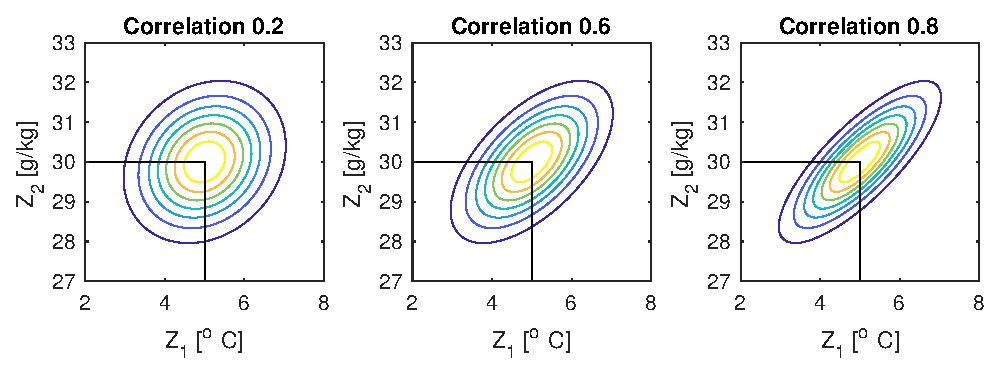
\includegraphics[width=0.99\textwidth]{Figures/illus_bivar.eps}
  \caption{Density contour plots having different correlations between
    temperature and salinity. The densities have unit variance and the thresholds are identical to the mean values $5^o C$ and $30 mg/l$.}\label{illus_bivarDens} 
\end{figure}
Here, the thresholds are set equal to the mean, $\mu_a=t_a=5^o C$ and salinity $\mu_b=t_b=30$ mg/l. The displayed densities have unit standard deviations for both temperature and salinity, but we also study the effect of doubling the standard deviations. 

Table \ref{tab:sim_rhoab} shows the EPs and the associated Bernoulli variance (second row) for the examples indicated in Fig. \ref{illus_bivarDens}. The EPs increase with the correlation as there is a stronger tendency of having jointly small temperature and salinity. The Bernoulli variance is similarly largest for high correlation. EPs and Bernoulli variances are the same for standard deviation $1$ or $2$, and this means that high variability in the temperature and salinity variables is not captured in the $p(1-p)$ expression.

\begin{table}[!h] \centering \caption{EP and Bernoulli variance for different correlations and variances (top rows), and expected Bernoulli variances for both data 
    and only for temperature (bottom rows).}
  \begin{tabular}{c|ccc|ccc}
 &\multicolumn{3}{c}{$\sigma_b=\sigma_a=1$} & \multicolumn{3}{c}{$\sigma_b=\sigma_a=2$} \\
\hline
Correlation $\gamma$ & 0.2 & 0.6 & 0.8 & 0.2 & 0.6 & 0.8 \\
\hline
$p$ & 0.28 & 0.35 & 0.40 & 0.28 & 0.35 & 0.40 \\ 
$p(1-p)$ & 0.20 & 0.23 & 0.24 & 0.20 & 0.23 & 0.24 \\ 
$E_{(y_a,y_b)}(p (1-p))$ & 0.092 & 0.089 & 0.085 & 0.052 & 0.051 & 0.049 \\ 
$E_{y_a}(p (1-p))$ & 0.151 & 0.138 & 0.123 & 0.137 & 0.114 & 0.093 \\ 
\hline
\end{tabular}
\label{tab:sim_rhoab}
\end{table}

Table \ref{tab:sim_rhoab} (bottom two rows) shows results of expected Bernoulli variance calculations. This is presented for a design gathering both data types $(y_a,y_b)$, and for a design with temperature measurements $y_a$ alone. Having both data; $(y_a,y_b)^t=(\xi_a,\xi_b)^t+N(0,0.5^2\bI)$, while $y_a=\xi_a+N(0,0.5^2)$ when only temperature is measured.
The results in Table \ref{tab:sim_rhoab} shows that 
the expected Bernoulli variance gets lower with larger standard deviations $\sigma_a$ and $\sigma_b$ (right columns). The reduction of Bernoulli variance is largest for the cases with high correlation $\gamma$. Albeit smaller, there is also uncertainty reduction when only temperature is measured (bottom row), especially when the temperature and salinity are very dependent. When correlation is low ($\gamma=0.2$) there is hardly any information about salinity in the temperature data, and hence less uncertainty reduction. In the application with fresh cold water from the river, the temperature and salinity variables will not only be interdependent, but they will be dependent in the spatial dimension. This dependence will also impact design criteria when we evaluate the information measure by integrating over several locations $\bx$. 

%\subsection{Expected classification criteria}

%{\bf{I have not done anything here - skip this, I think}}.

%Rather than minimizing expected variance one can aim at minimizing the classification probability of the excursion set: 
%$\min [p,(1-p) ]$, see e.g. \cite{lilleborge2016information}. 

%Again, since the conditional mean is a linear in the data, we only have to look at the %relevant linear combination via $\bm_{\xi}=E(\bxi)$.
%See also \cite{bhattacharjya2013value}.

%\begin{equation}
%E(\min \{ p,(1-p)\})=\int \min P(\xi_a \leq t, \xi_b \leq s),[1-P(\xi_a \leq t, \xi_b \leq s)] p(E(\bxi)=) dE(\bxi)=,
%\end{equation}
%for the complementary probabilities, this is again evaluated by the corner regions for the block, and $\Phi_4()$ evaluations are required.

%In the end, this result is integrated over the spatial domain $x \in X$.

\section{Sequential updating and heuristic path planning}\label{sec:heuristics}

Recall that the AUV can adapt its survey plan based on what it is measuring, in accordance with the sense, plan, act loop (Fig. \ref{fig:sense-plan-act}). Here we present adaptive strategies for sampling.

\subsection{Optimal sequential design}
\label{myopic}

An adaptive AUV survey is split in many rounds (stages), and at each round, the survey design is found by considering the largest reduction in uncertainty of the ES. In our setting the selection is made on the graph defined by the nearest grid nodes in the domain $\mathcal{M}_g$.

The optimal sequential design does not only consider the best current AUV grid node, but also what data gathered at this node would lead to for future sampling at the next stages. 
Let $d^{j,s}$ denote design number $j$ at stage $s$ of sequential surveying. If this design is selected, data $\by^{j,s}$ will be gathered. The optimal path selection situation is then depicted in Figure \ref{fig:PathSelOpt}, 
\begin{figure}[h!]
\centering
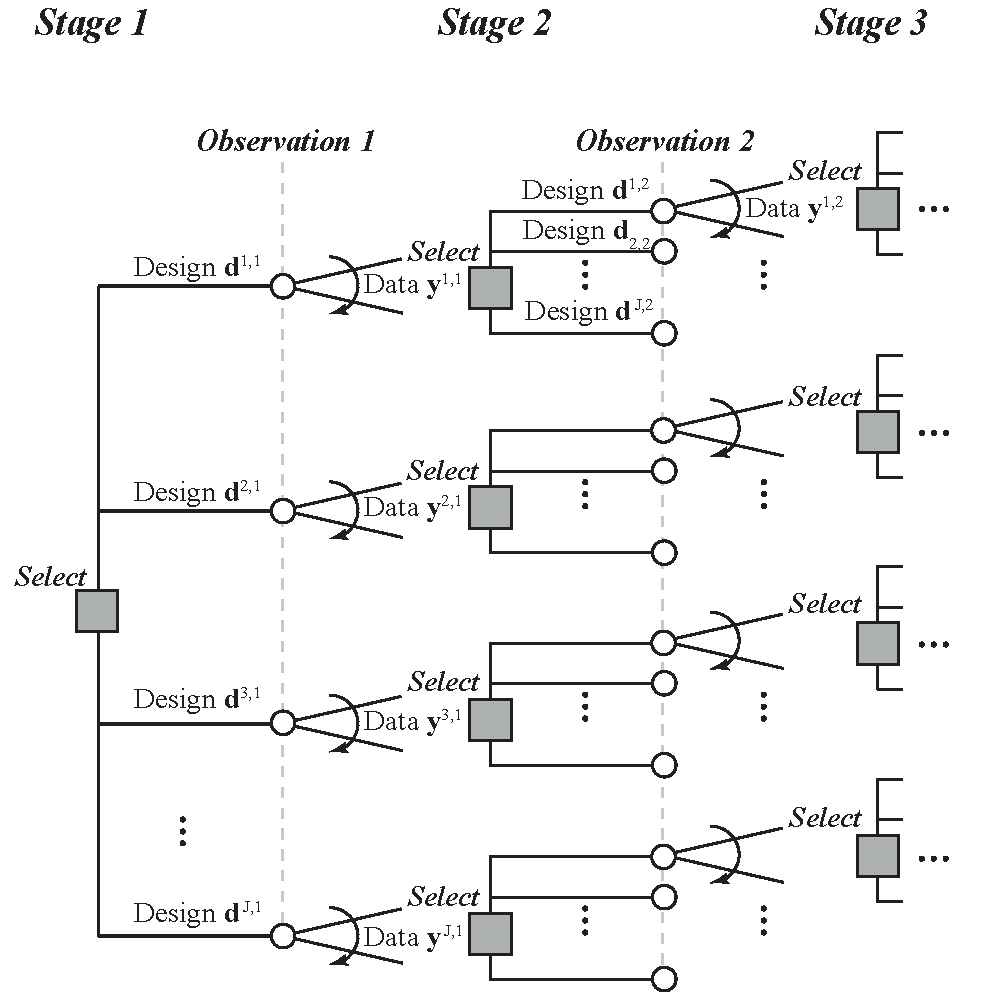
\includegraphics[width=0.85\textwidth]{Figures/sequent_select.pdf}
\caption{Optimal sequential path selection.}\label{fig:PathSelOpt}
\end{figure}
where design choices are indicated by squares while data realizations are indicated by circles. 
%terms this optimal design is defined as
%\begin{equation}\label{opt_crit}
%    \bd^* = \mbox{argmin}_{d^{j,1}} \left\{ \int_{\by^{j,1}} \mbox{argmin}_{d^{j,2}} \left\{ \int_{\by^{j,2}} \ldots \pi(\by^{j,2}|\by^{j,1}) d\by^{j,2} \right\} \pi(\by^{j,1}) d \by^{j,1} \right\},
%\end{equation}
%where $\ldots$ represents the expected variance reduction in the ES under the continued optimal design, which will depend on the data at earlier stages. 
The mathematical expression for the optimal design then involves a series of intermixed maximizations over designs and integrals over data.
In practice the optimal solution is not tractable because of the enormous growth over stages, see e.g. \cite{sucar2015probabilistic} and \cite{powell2016perspectives}. 

Instead, we next outline heuristic strategies. In terms of notation, let $\mathcal{Y}^{s-1} =\{d^{j,r}, \by^{j,r} ; r=1,\ldots,s-1 \}$ denote the data gathered until stage $s-1$, using a selected design $d^{j,r}$, $r=1,\ldots,s-1$. 

The derived closed form solutions for the expected IBV are still important building blocks when constructing the sampling designs as they will be used to score the different adaptive design. Efficient calculation is important for using adaptive survey designs with robotic platforms. 
 
\subsection{Naive path planning}
\label{naive}

The simplest heuristic for adaptive sampling is to choose the next sampling location based on current EPs. The variance is largest for EPs equal to $0.5$, so one selects the design location with EP closest to $0.5$. 

At stage $s$, based on the currently available data $\mathcal{Y}^{s-1}$, we fit an updated Gaussian model from Eq. (\ref{gp_upd}), with mean $\bm_{s-1}=E(\bxi|\mathcal{Y}^{s-1})$ and covariance matrix $\bS_{s-1}=\mbox{Var}(\bxi|\mathcal{Y}^{s-1})$. 
The next round of measurements $\by^{j,s}$, can be gathered with design $d^{j,s}$, $j=1,\ldots,J$, where $J$ indicates all possible AUV directions or paths at the current stage. The {\it{naive}} strategy selects the design according to
\begin{eqnarray}\label{critNaive}
    d^{*,s} &=& \mbox{argmin}_{j \in \{1,\ldots,J\}} |p(\bx_{d^{j,s}};\mathcal{Y}^{s-1})-0.5|, \\
    p(\bx;\mathcal{Y}^{s-1}) &=& P(\xi_a(\bx) \leq t_a, \xi_b(\bx) \leq t_b | \mathcal{Y}^{s-1}). \nonumber
\end{eqnarray}
This strategy does not account for the uncertainty in the temperature or salinity variables, only if one design (node) has EPs closer to $0.5$ (see Table \ref{tab:sim_rhoab}, line two). Neither does it account for spatial correlation. This strategy lacks memory of where it has been and where the uncertainty has been reduced. For this reason it can easily get stuck in local regions. 

\subsection{Myopic path planning}
\label{myopic}

The myopic (greedy) strategy which we present here is optimal if we imagine taking only one more round of measurements. In this selection strategy there is no anticipation of what the subsequent designs might offer, beyond the first round. 

Based on the currently available data $\mathcal{Y}^{s-1}$, we again fit an updated Gaussian model, represented on the grid locations covering the spatial domain. 
The next round of measurements $\by^{j,s}$, can be gathered with design $d^{j,s}$, $j=1,\ldots,J$, indicating all possible AUV directions / paths at the current stage. The selected design is then
\begin{eqnarray}\label{critSEQ}
    d^{*,s} &=& \mbox{argmin}_{j \in \{1,\ldots,J\}} \left\{ V_{m,\mbox{upd,j}} \right\},  \\
V_{m,\mbox{upd}} & \approx & \sum_{\bx \in \mathcal{M}_g} E_{\by^{j,s}|\mathcal{Y}^{s-1}} \left\{ p(\bx;\mathcal{Y}^{j,s})\left( 1-p(\bx;\mathcal{Y}^{j,s})\right) \right\} \Delta, \nonumber \\
    p(\bx;\mathcal{Y}^{j,s}) &=& P(\xi_a(\bx) \leq t_a, \xi_b(\bx) \leq t_b |\by^{j,s},\mathcal{Y}^{s-1}). \nonumber
\end{eqnarray}

Note that this strategy gives a sequential conditional version of the formula in Eq. (\ref{sur}). Now $\mathcal{Y}^{s-1}$ is available, and the expectation is with respect to the conditional density $\pi(\by^{j,s}|\mathcal{Y}^{s-1})$. A similar closed form calculation for expected IBV is hence applicable in Eq. (\ref{critSEQ}), using the updated GP model from step $s-1$. 
Once the data are collected for the best design, the GP model is updated again. The mean $\bm_{s}$ and covariance matrix $\bS_{s}$ are used to compute the next design at stage $s+1$, and so on. 

Even though this myopic strategy is non-anticipative, it still gives a reasonable approach for creating designs in many applications. Moreover, it is easily implemented on-board an AUV, using the efficient approach for data updating of the GP model and the calculation of the closed form expected IBV expressions for each next survey line.


\subsection{Look-ahead path planning}
\label{LA}

We now extend the myopic strategy to a look-ahead strategy which is optimal when one can gather only two more rounds of measurements. In addition to the next round of measurements $\by^{j,s}$, this look-ahead strategy hence anticipates the subsequent design $j_2$ with data $\by^{j_2,s+1}$, when choosing the current design $d^{j,s}$. 
The selected design is
\begin{eqnarray}\label{critLA}
    d^{*,s} &=& \mbox{argmin}_{j \in \{1,\ldots,J\}} \left\{ U_{la,\mbox{upd,j}} \right\},  \\
    U_{la,\mbox{upd},j} & = &  E_{\by^{j,s}|\mathcal{Y}^{s-1}} \left\{ \mbox{argmin}_{j_2 \in \{1,\ldots,{J}_2\}} \left[ V_{la,\mbox{upd},j_2} \right] \right\}, \nonumber \\
V_{la,\mbox{upd},j_2} & \approx & \sum_{\bx \in \mathcal{M}_g} E_{\by^{j_2,s+1}|\mathcal{Y}^{j,s}} \left\{ p(\bx;\mathcal{Y}^{j,s+1})\left( 1-p(\bx;\mathcal{Y}^{j,s+1})\right) \right\} \Delta, \nonumber \\
    p(\bx;\mathcal{Y}^{j,s+1}) &=& P(\xi_a(\bx) \leq t_a, \xi_b(\bx) \leq t_b |\by^{j_2,s+1},\mathcal{Y}^{j,s}). \nonumber
\end{eqnarray}
Here, $\mathcal{Y}^{j,s}=\{\by^{j,s},\mathcal{Y}^{s-1}\}$ and $\mathcal{Y}^{j,s+1}=\{\by^{j_2,s+1},\mathcal{Y}^{j,s}\}$ represent the sets of data variables, and the expectations are with respect to the conditional densities $\pi(\by^{j,s}|\mathcal{Y}^{s-1})$ and $\pi(\by^{j_2,s+1}|\by^{j,s},\mathcal{Y}^{s-1})$. 

Because of the intermixed optimization and expectation, there is no longer a closed form for the required integrals. Instead, we solve the first expectation by Monte Carlo sampling of data $\by^{j,s}$ from its conditional distribution. For each data sample, the second expectation is solved using the closed form expressions for expected IBV from Section \ref{sec:sur}. 

Even though the strategy looks at two stages, it is only used to find the current best design. When data are collected, the GP model is updated, and the mean $\bm_{s}$ and covariance matrix $\bS_{s}$ are used to compute the next design at stage $s+1$, now anticipating what stage $s+2$ could offer, and so on. 

This look-ahead approach is much more computer-demanding than the myopic strategy, and for practical implementation we prune paths in the evaluation of Eq. (\ref{critLA}). This means that we do not compute all possible branches of the first two stages, as they are indicated in Figure \ref{fig:PathSelOpt}. Instead, we use the myopic strategy to rank the three best designs on the first stage alone, and for each of these we go through with the look-ahead calculation. 

\section{Simulation study}\label{sec:simulations}

Results from tests performed to study the properties of different static and sequential survey designs, in a realistic simulated case, is shown in this section. The context is mapping a freshwater plume defined by a temperature and salinity field using an AUV. 

\subsection{Modeling}

We use a bivariate GP model for temperature and salinity, where we specify the prior mean 
\begin{equation}\label{m}
    \bmu(\bx)=E 
    \begin{bmatrix}
    \xi_a(\bx) \\
    \xi_b(\bx) 
    \end{bmatrix}=\begin{bmatrix} \mu_{a}(\bx)\\
\mu_{b}(\bx)
\end{bmatrix} 
= \begin{bmatrix} \beta_{a,0} + \beta_{a,1} x_{\mbox{East}} \\
\beta_{a,1} + \beta_{b,1} x_{\mbox{East}}
\end{bmatrix}.
\end{equation}
In this simulation setup, which is motivated by the real case, we expect the eastern part of the domain to be cold freshwater. This situation mimics that of a river mouth entering from the south, and the water masses are pulled to the east. The actual trends are in practice set from preliminary information or runs of oceanographic models solving the differential equations for fluid flow. In this example the mean is specified by $\beta_{a,1}=0.065$ and $\beta_{b,1}=0.1$. Further, the intercepts of the temperature and salinity variables are set to $\beta_{a,0}=5.8$ and $\beta_{b,1}=29.0$. 

%The prior assumption used by the agent are $\tilde{\beta_{a,1}}=0.085$ and $\tilde{\beta_{b,1}}=0.138$, which assumes that the process is centered. 

The covariance is assumed to be stationary and separable for the two variables. 
The $2 \times 2$ pointwise covariance matrix is set to
\begin{equation}\label{v0}
\bSigma(\bx)=\mbox{Var} 
\begin{bmatrix}
    \xi_a(\bx) \\
    \xi_b(\bx) 
    \end{bmatrix}=
\begin{bmatrix}
0.25^2 & 0.6 \cdot 0.25^2 \\
0.6 \cdot 0.25^2 & 0.25^2
\end{bmatrix}.
\end{equation}
The spatial correlation is of a Matern type giving
\begin{equation}\label{v}
\mbox{Corr} 
\left(
\begin{bmatrix}
    \xi_a(\bx) \\
    \xi_b(\bx) 
    \end{bmatrix},
    \begin{bmatrix}
    \xi_a(\bx') \\
    \xi_b(\bx') 
    \end{bmatrix}
    \right)
    = \begin{bmatrix}
1 & 0.6  \\
0.6  & 1
\end{bmatrix}(1+\phi |\bx-\bx'|)\exp (-\phi |\bx-\bx'|),
\end{equation}
and $\phi=0.3$ indicates an effective correlation range of about $1200$ m. 
%Figure \ref{fig:stat_design} shows the contour lines for the EP for the reference. We notice the trend of increasing salinity and temperature to the west.  
We study sensitivity to the parameter specification in the results below.
One realization of the random fields representing salt and temperature is shown in Figure \ref{fig:true_temp} and \ref{fig:true_sal}. The true ES from this prior realization is plotted in Figure \ref{fig:ESet}.

\begin{figure}[!h]
  \centering
  \subfigure[Simulated temperature.]{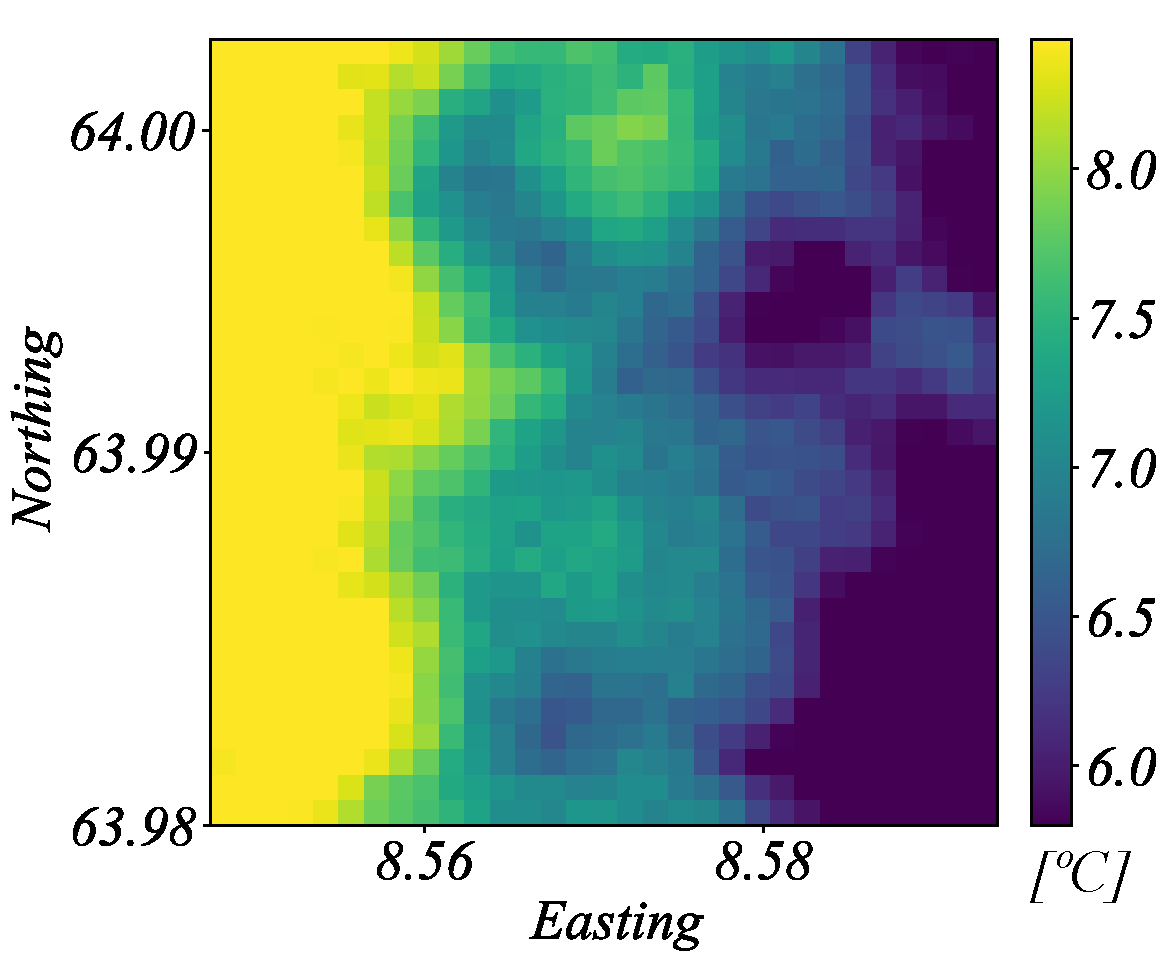
\includegraphics[height = 0.40\textwidth]{Figures/sim/true_temp.pdf}\label{fig:true_temp}}
  \hfill
  \subfigure[Simulated salinity.]{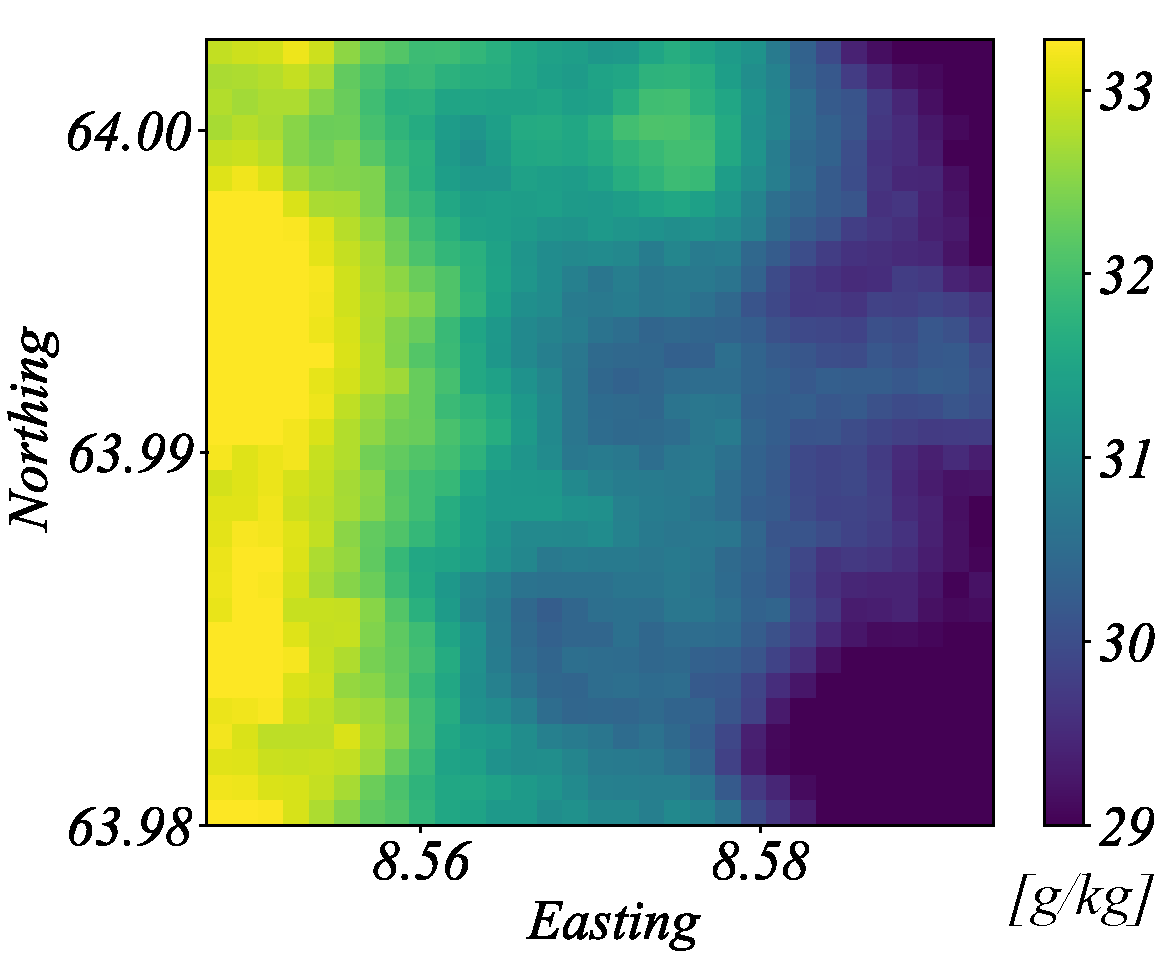
\includegraphics[height = 0.40\textwidth]{Figures/sim/true_sal.pdf}\label{fig:true_sal}}
  \hfill
  \subfigure[Excursion set given the realization of temperature and salinity.]{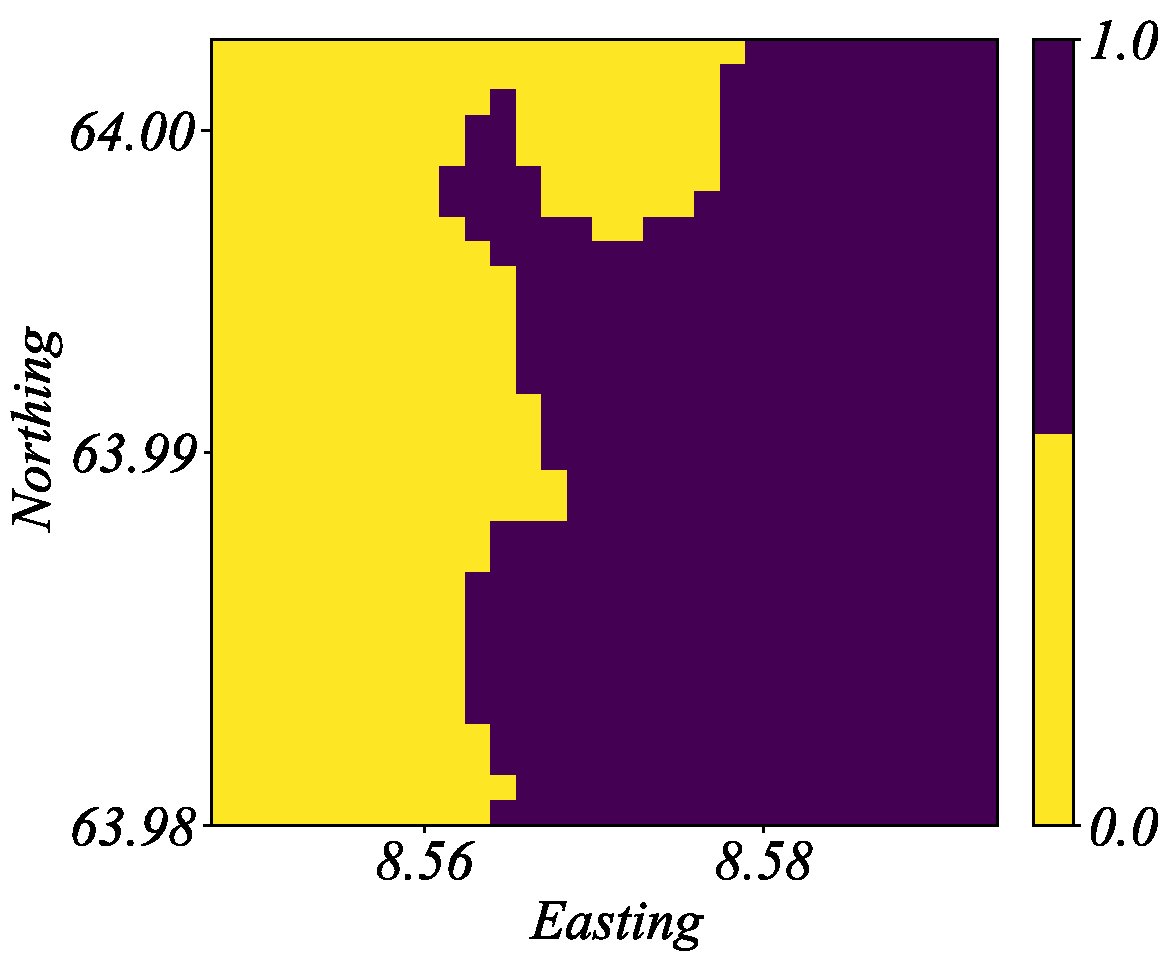
\includegraphics[height = 0.40\textwidth]{Figures/sim/es_ts_true.pdf}\label{fig:ESet}}
  \hfill
  \subfigure[Excursion probabilities given collected data along the strategy ``static\_north".]{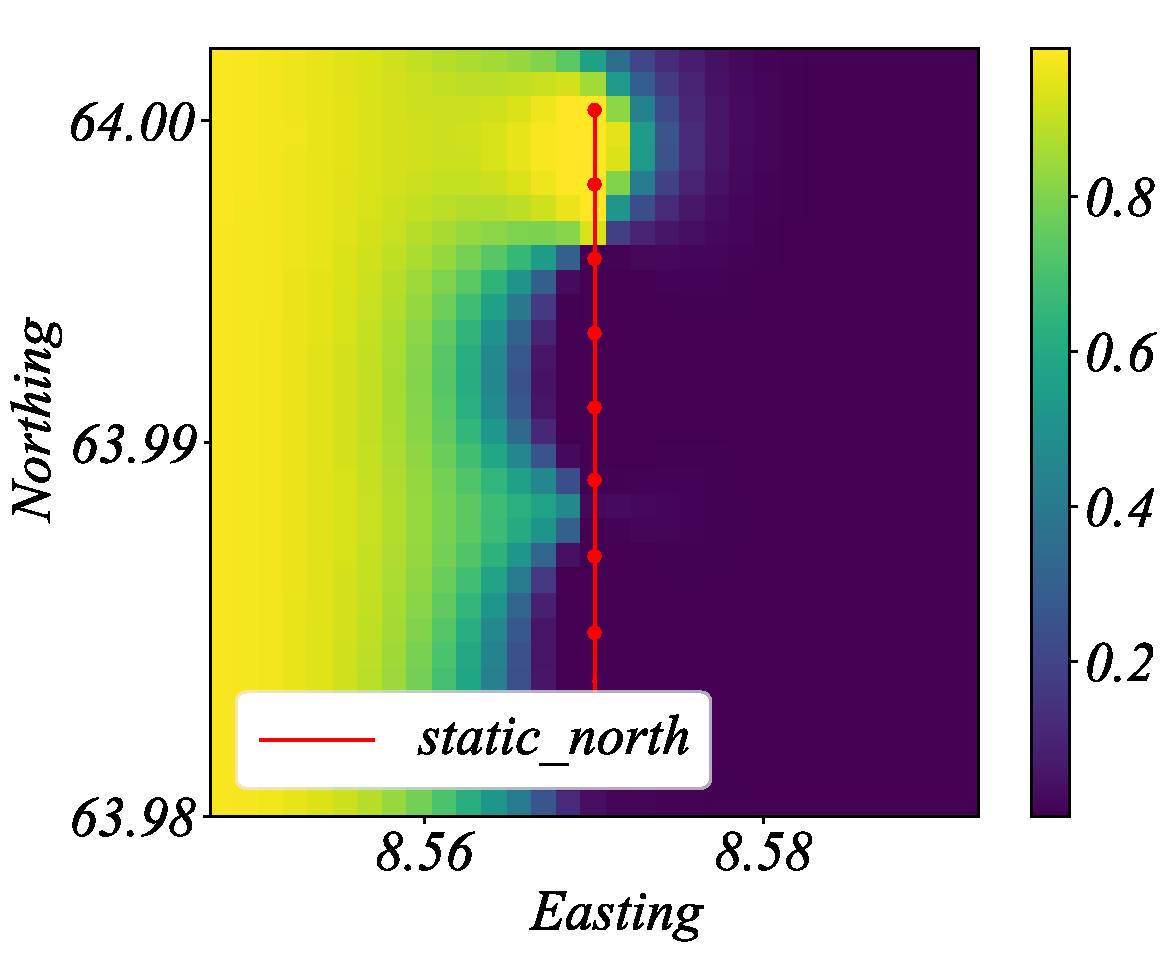
\includegraphics[height = 0.40\textwidth]{Figures/sim/es_ts_posterior.pdf}\label{fig:Eprob}}
  \caption{\ref{fig:true_temp} and \ref{fig:true_sal} shows
    realisations of the simulated temperature and salinity fields, as
    well as the associated excursion set \ref{fig:ESet}.
    \ref{fig:Eprob} show the estimated excursion probabilities after
    performing data collection along the N-S survey line.} 
\label{fig:realisations}
\end{figure}

\newpage
\subsection{Static and sequential sampling designs}\label{sec:sampling_designs}

%Three different designs are considered as indicated in Figure \ref{fig:stat_design}. 
%\begin{figure}[h!]
%\centering
%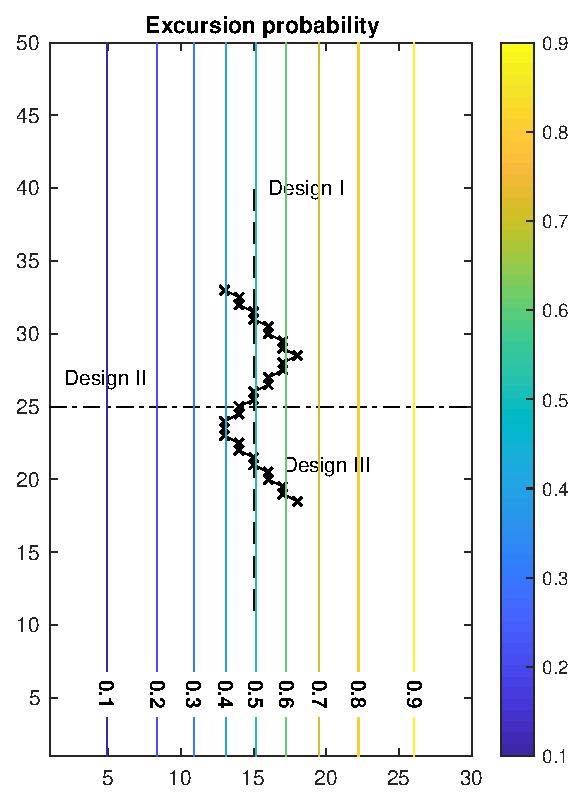
\includegraphics[width=0.65\textwidth]{Figures/Des3.eps}
%\caption{Three different static survey designs plotted on the initial EP.}\label{fig:stat_design}
%\end{figure}
%In this display the designs are plotted along with the prior probability contours of the ES for the reference parameter inputs. 

We compare three different static designs denoted \texttt{static\_north}, \texttt{static\_east and} \texttt{static\_zigzag} with the three sequential approaches \texttt{naive}, \texttt{myopic}, and \texttt{look-ahead}. The static sampling paths are pre-determined and cannot be changed on the basis of data, representing the archetypical pre-planned observation strategies used in current observational practices. For a fixed survey length, the expected variance after static surveying is analytically available (equal coverage each time), but here we focus on the properties from the sequential designs which are evaluated using Monte Carlo sampling over several replicates of realizations from the prior, and conducting simulated sequential surveying for each one; making the result dependent on the observed data. For comparison, the same setup is used for the static designs. Figure \ref{fig:Eprob} shows the conditional EP, given data gathered along the north-south survey line for the realization indicated in these displays. In the Monte Carlo replicates, such results are repeatedly computed to approximate the expected variance reduction in the ES. Along with this criterion we also compare predictive performance measured by root mean square error (RMSE) in the temperature and salinity fields and variance reduction in these two field variables. It is important to note that the objective function used by the agents is focused on reducing the expected variance in the ES, but we nevertheless hope to achieve good predictive performance for criteria such as RMSE as well. Another non-statistical criteria that is important for practical purposes is the computing time of the strategy, as this will impact the performance of the approach in the field for an embedded system. 

The sequential sampling agents start at the center East-West coordinate at the southern end of the domain (node 53), see Fig. \ref{fig:wp_graph}.

\begin{figure}[h]
\centering
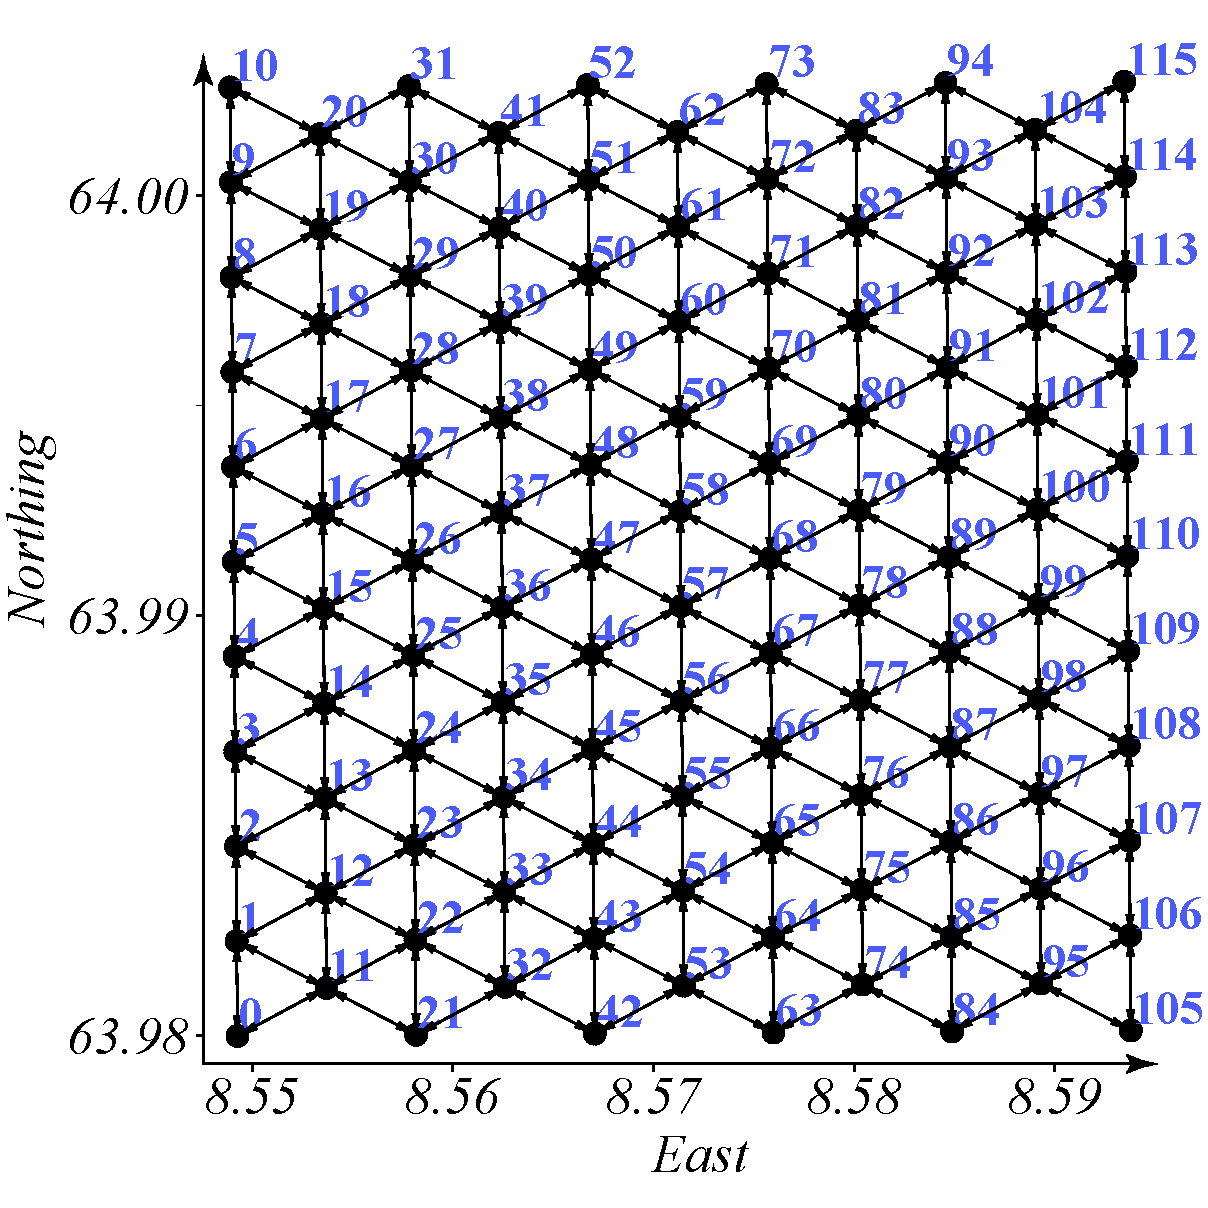
\includegraphics[width=0.50\textwidth]{Figures/sim/wp_graph_paper.pdf}
\caption{The equilateral waypoint graph used to discretize the route choices over the $31\times31$ grid.}
\label{fig:wp_graph}
\end{figure}

Maintaining the AUV example, the AUV will move along edges in the Fig. \ref{fig:wp_graph} waypoint graph. While doing so, the AUV will gather measurements. These are assimilated in the GP model, before an evaluation of the next node to sample will be conducted at the end of the edge. The paths of will differ for the various sequential designs due to the individual design criteria and the simulated variability in the environment among the replicates.

Results of the replicate runs are shown in Figure \ref{fig:sim_results},
where the different criteria are plotted as a function of surveying
distance. Here, expected ES variance in Figure \ref{fig:avg_ev} is
reduced most under the \texttt{myopic} and \texttt{look-ahead}
strategies, performing almost equally.

\begin{figure}[!th]
  \centering
  % \subfigure[Excursion set variance $E_{\by}(p[1-p])$.]{\label{fig:avg_ev}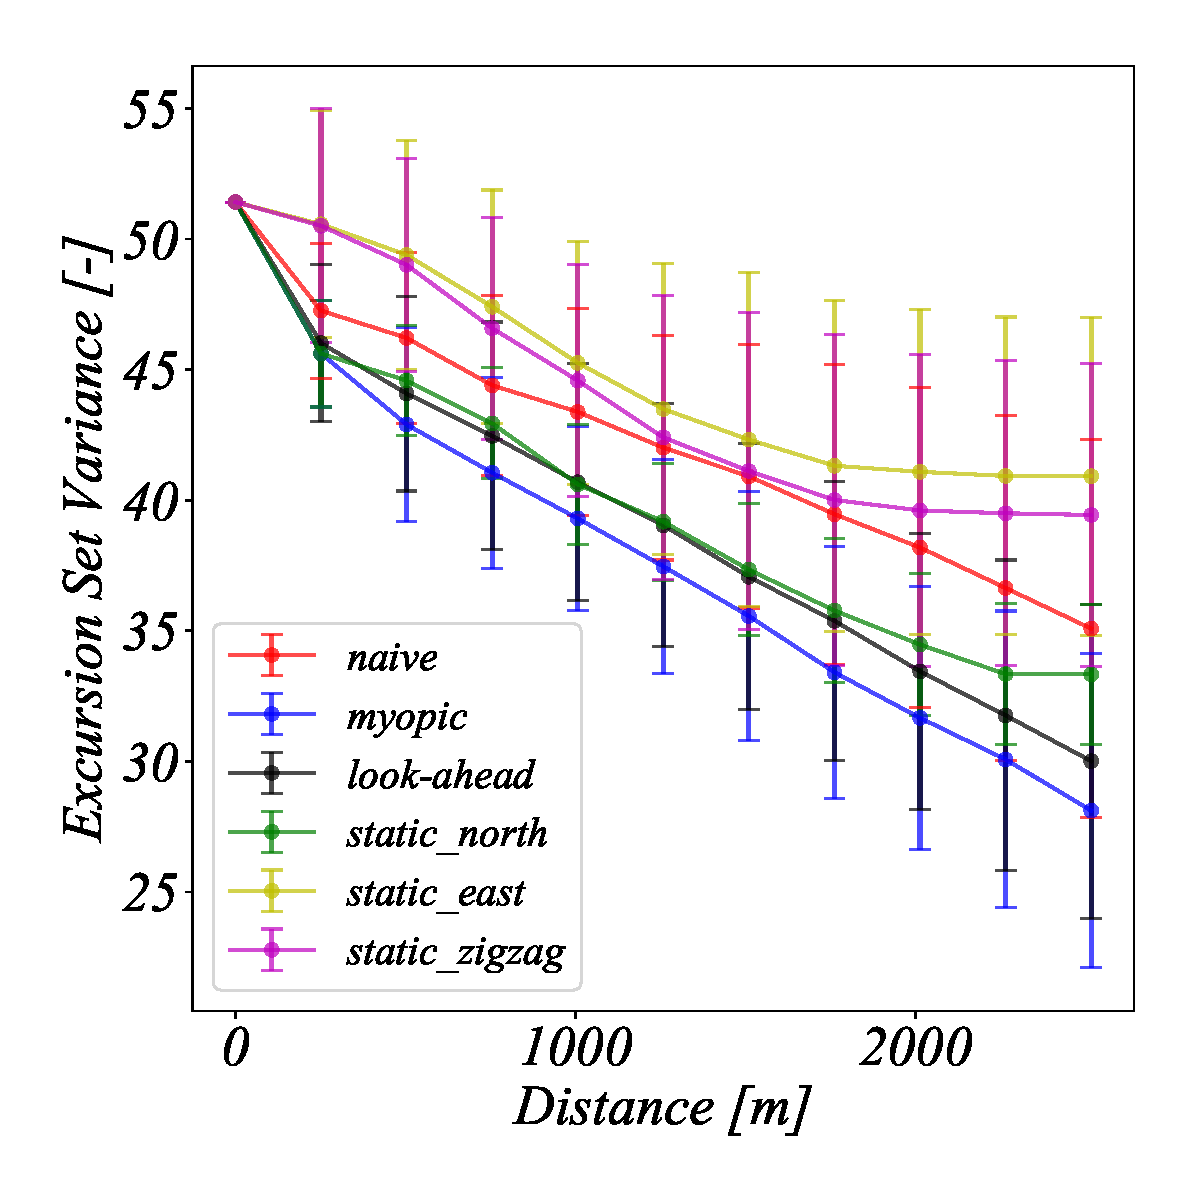
\includegraphics[height=0.49\textwidth]{Figures/sim/avg_EV.pdf}}
  \subfigure[Excursion set $E_{\by}$(p\lbrack 1-p\rbrack) variance.]{\label{fig:avg_ev}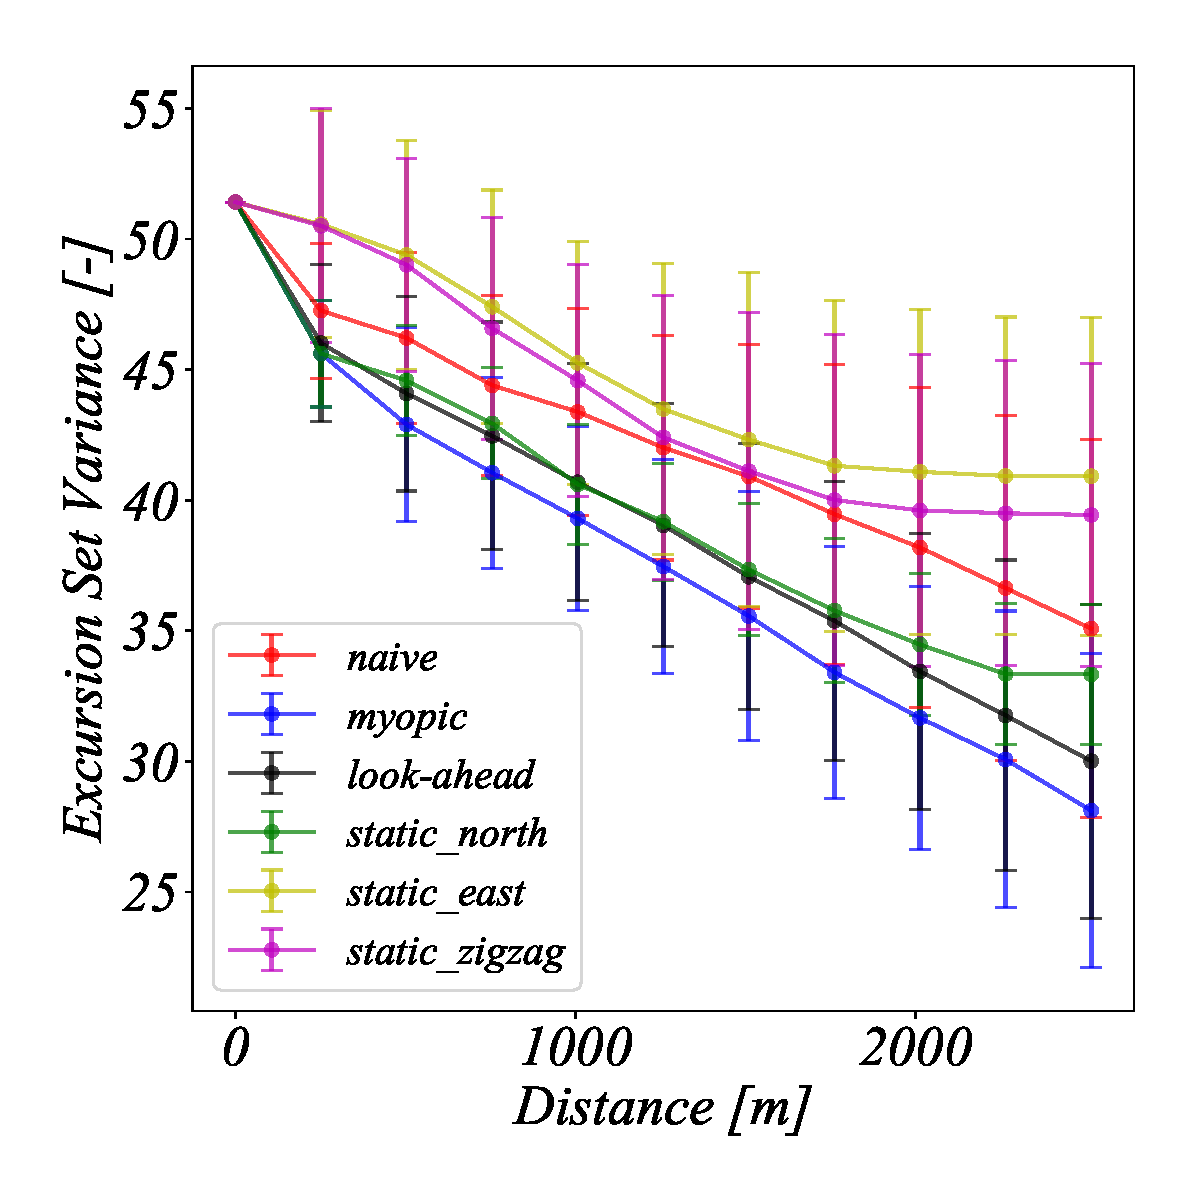
\includegraphics[height=0.49\textwidth]{Figures/sim/avg_EV.pdf}}
  \hfill
  \subfigure[RMSE between estimated field and truth.]{\label{fig:avg_rmse}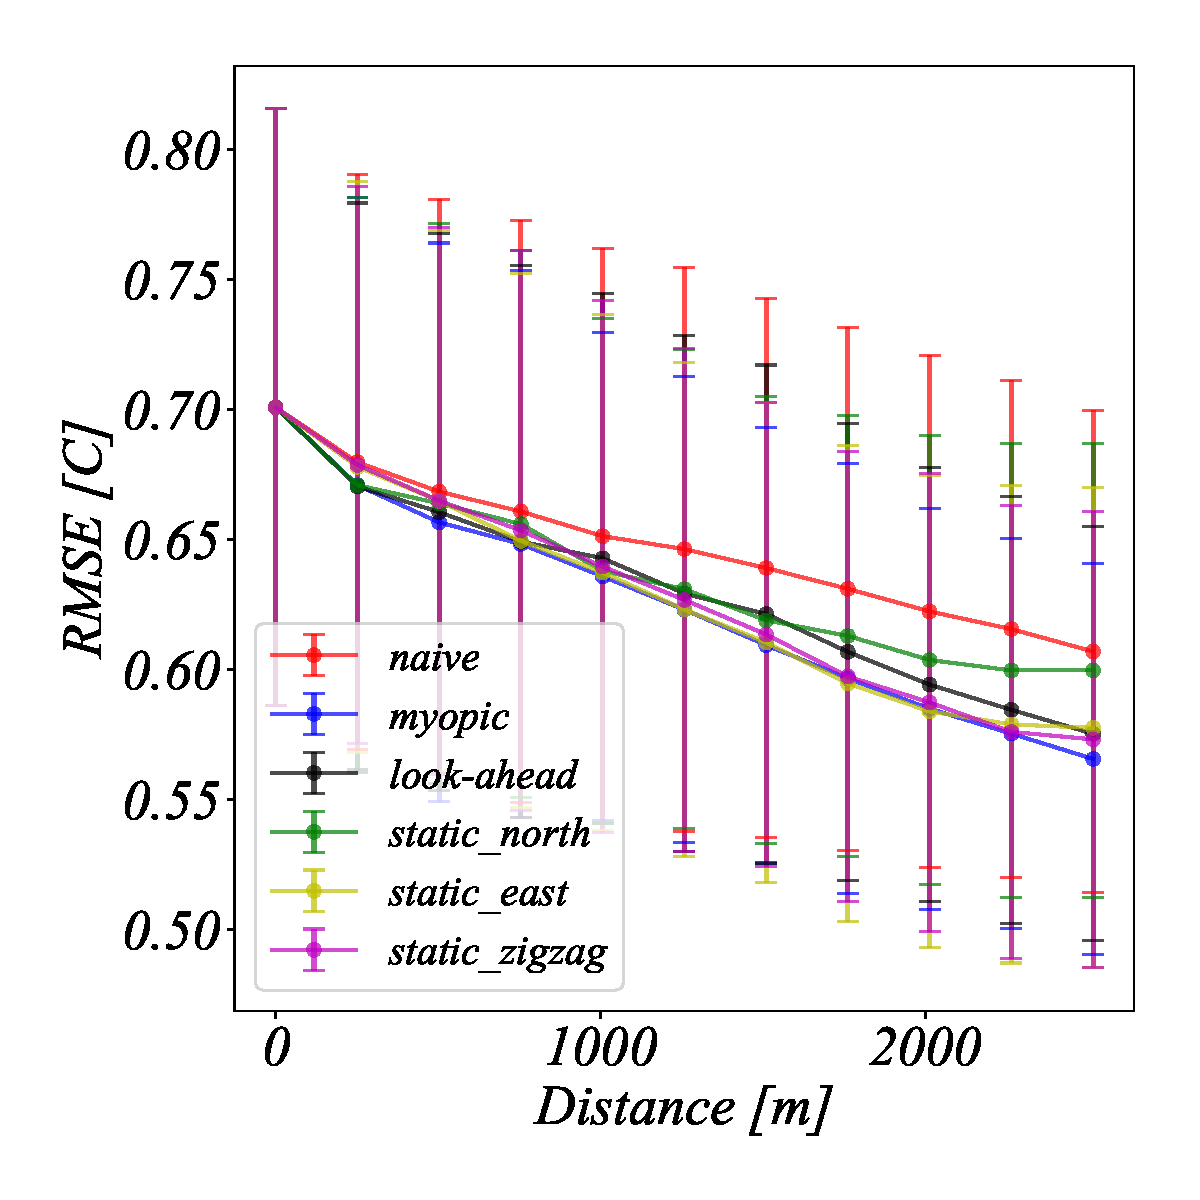
\includegraphics[height=0.49\textwidth]{Figures/sim/avg_RMSE.pdf}}
  \hfill 
  \subfigure[Explained variance $\bR^{2}$.]{\label{fig:avg_r2}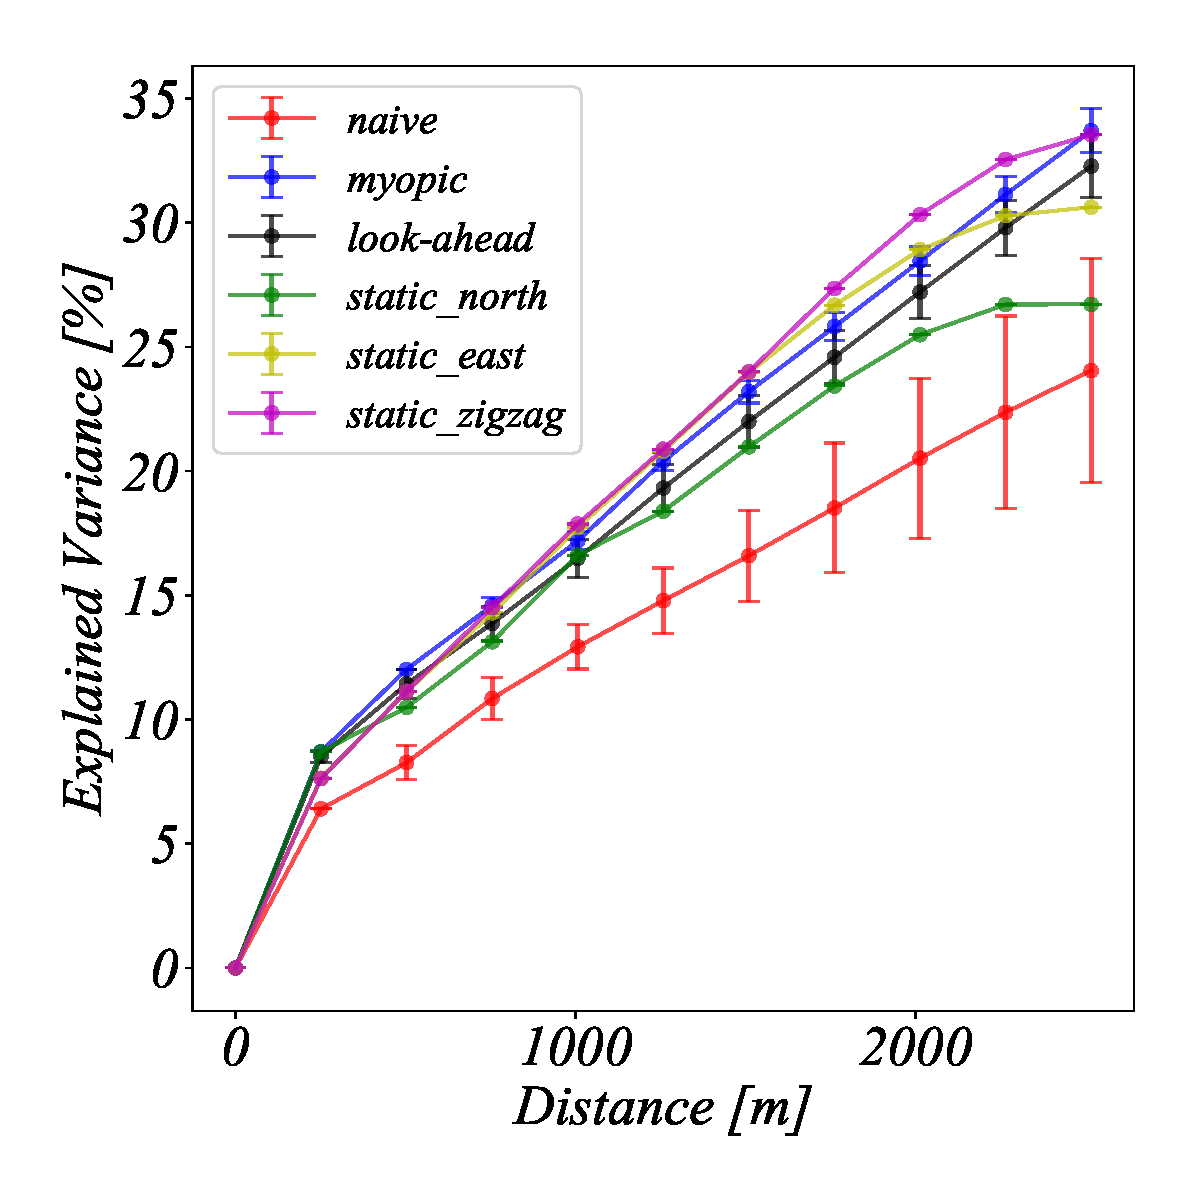
\includegraphics[height=0.49\textwidth]{Figures/sim/avg_R2.pdf}}
  \hfill 
  \subfigure[Time used to do inference.]{\label{fig:avg_time}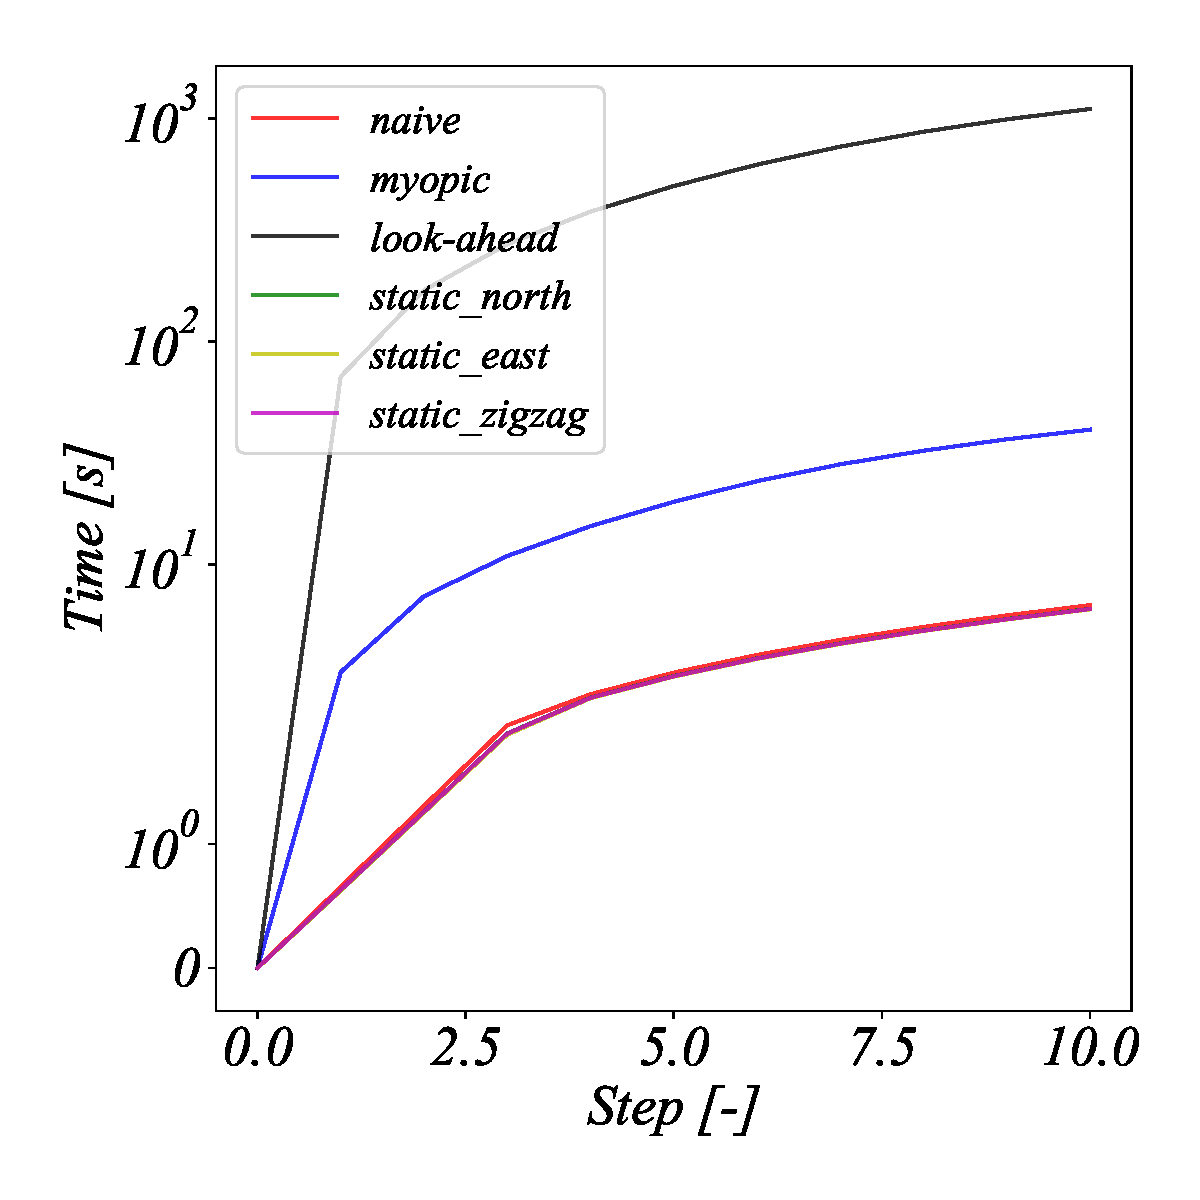
\includegraphics[height=0.49\textwidth]{Figures/sim/avg_Time.pdf}}
\caption{Simulation results from 100 replicate simulations for 10
  sampling choices/steps on the grid. (Updated:01.05.2019)} 
\label{fig:sim_results}
\end{figure}

The north-south design is also doing well, because it moves near the
boundary of the water masses. In Figure \ref{fig:avg_rmse} and
\ref{fig:avg_r2} we show results of RMSE and explained variance. Both
\texttt{myopic} and \texttt{look-ahead} still perform well, but some of
the static east and zigzag are also achieving good results because they
are set to always cover large parts of the domain, and in this way visit
locations that are not considered interesting by the sequential
strategies targeting ES variance. Regarding computing time in Fig.
\ref{fig:avg_time}, the \texttt{naive} strategy is on par with the
static designs, while \texttt{myopic} is slower and \texttt{look-ahead}
much slower. The \texttt{look-ahead} strategy is reaching levels that
are near impractical for on-board execution. Of course, with harder
pruning of branches in the graph, it would be faster to run. Then again,
this pruning is likely the reason that this strategy does not
outperforms the myopic approach. In Figure \ref{fig:route_choices} we plot the realized sampling paths of the sequential schemes and static designs.

\begin{figure}[!h]
  \centering
  \subfigure[Look-ahead strategy.]{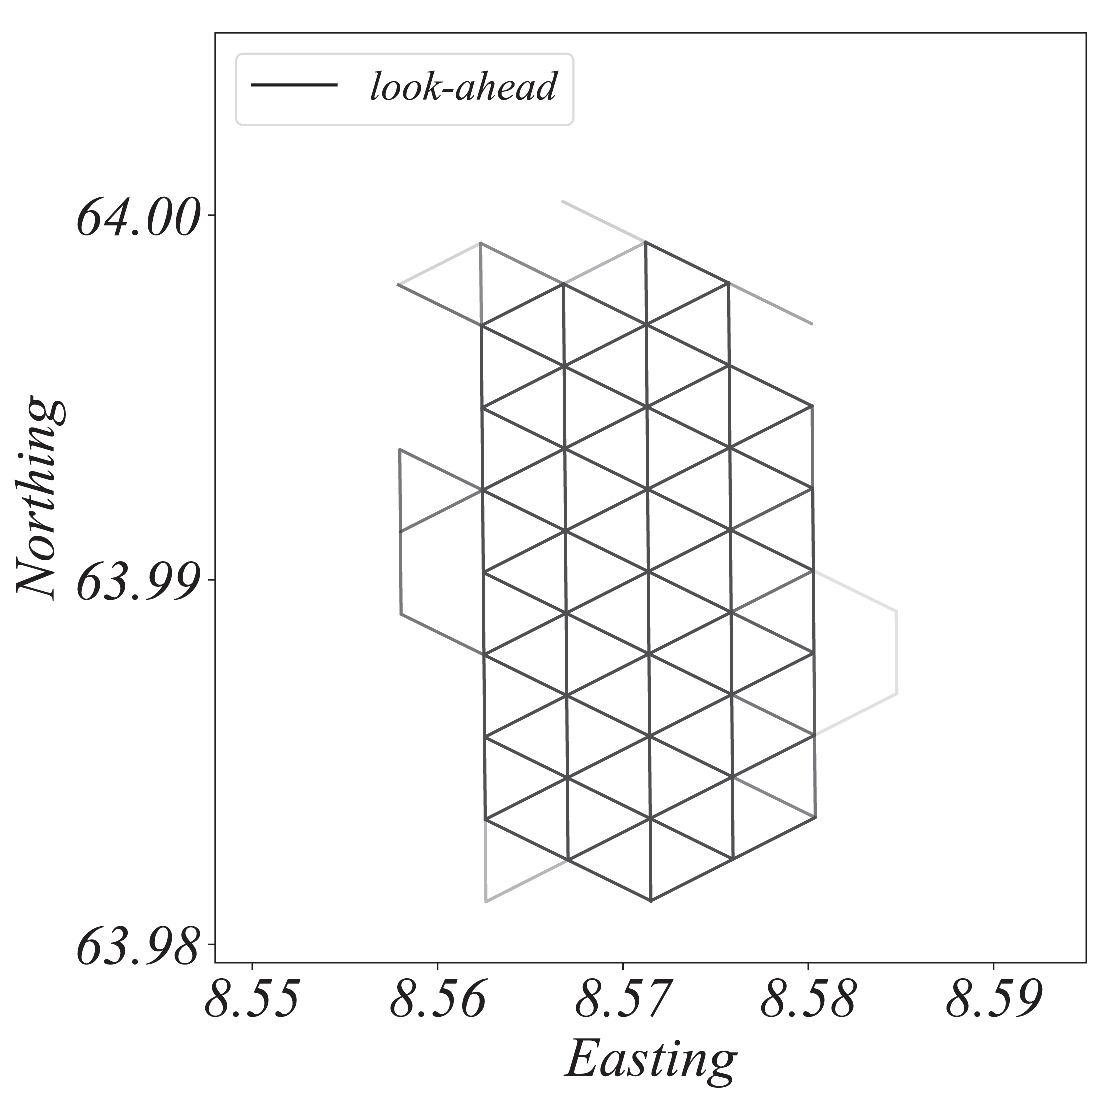
\includegraphics[height = 0.46\textwidth]{Figures/sim/route_look-ahead.pdf}\label{fig:avg_look-ahead}}
  \hfill
  \subfigure[Myopic strategy.]{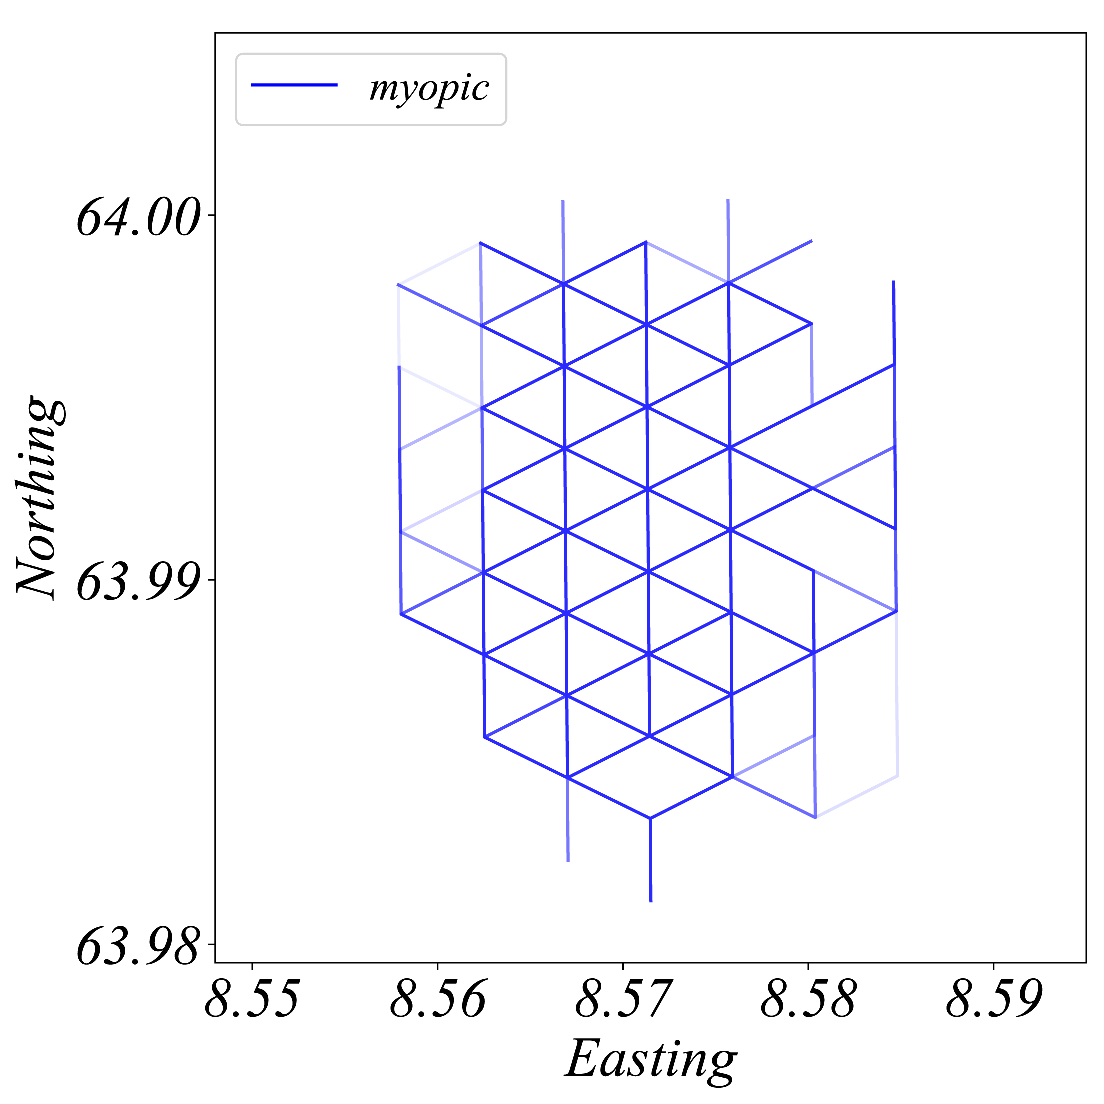
\includegraphics[height = 0.46\textwidth]{Figures/sim/route_myopic.pdf}\label{fig:avg_myopic}}
  \hfill
  \subfigure[Naive strategy.]{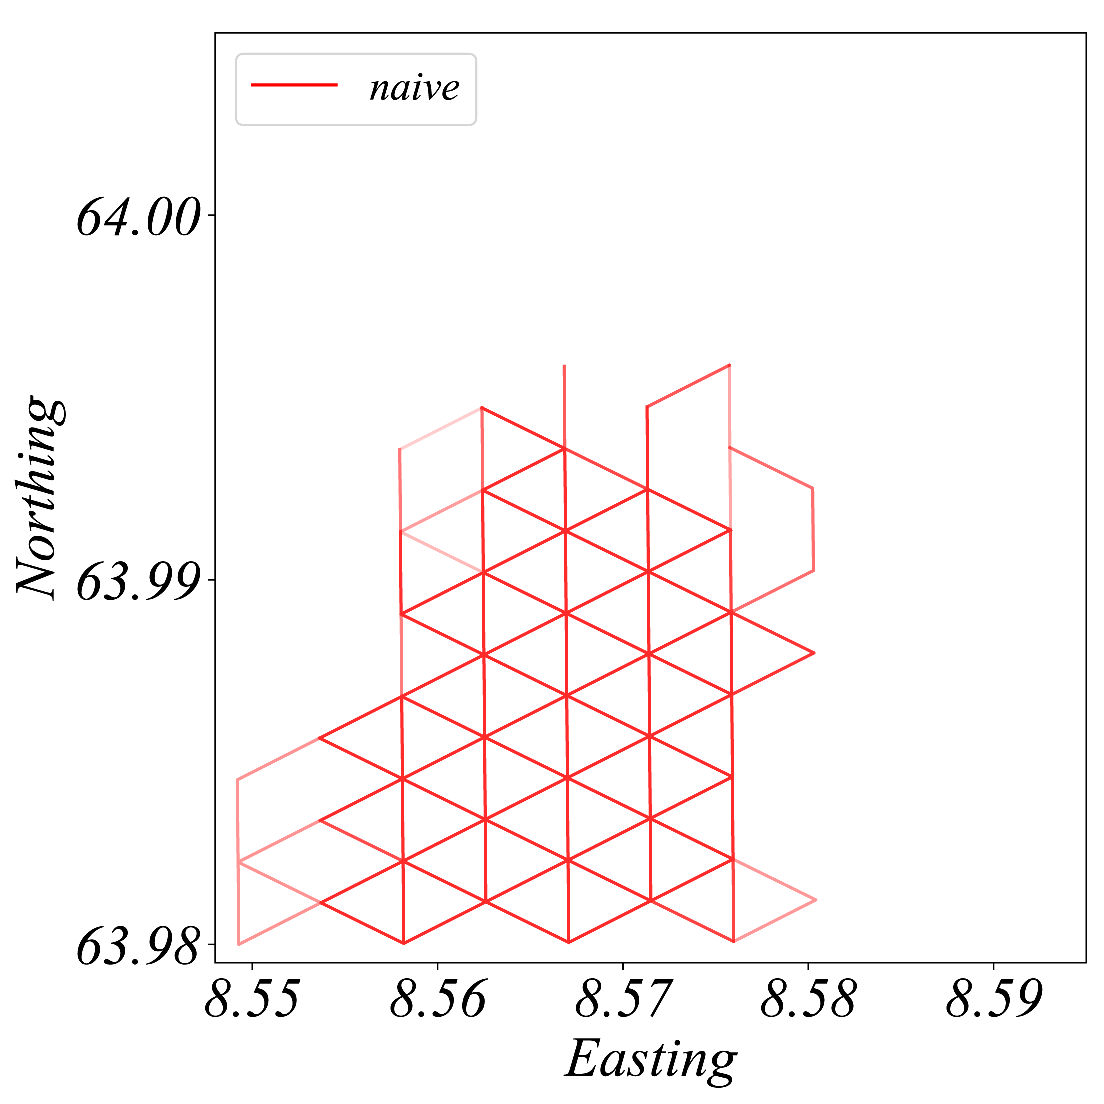
\includegraphics[height = 0.46\textwidth]{Figures/sim/route_naive.pdf}\label{fig:route_naive}}
  \hfill
  \subfigure[Static strategies.]{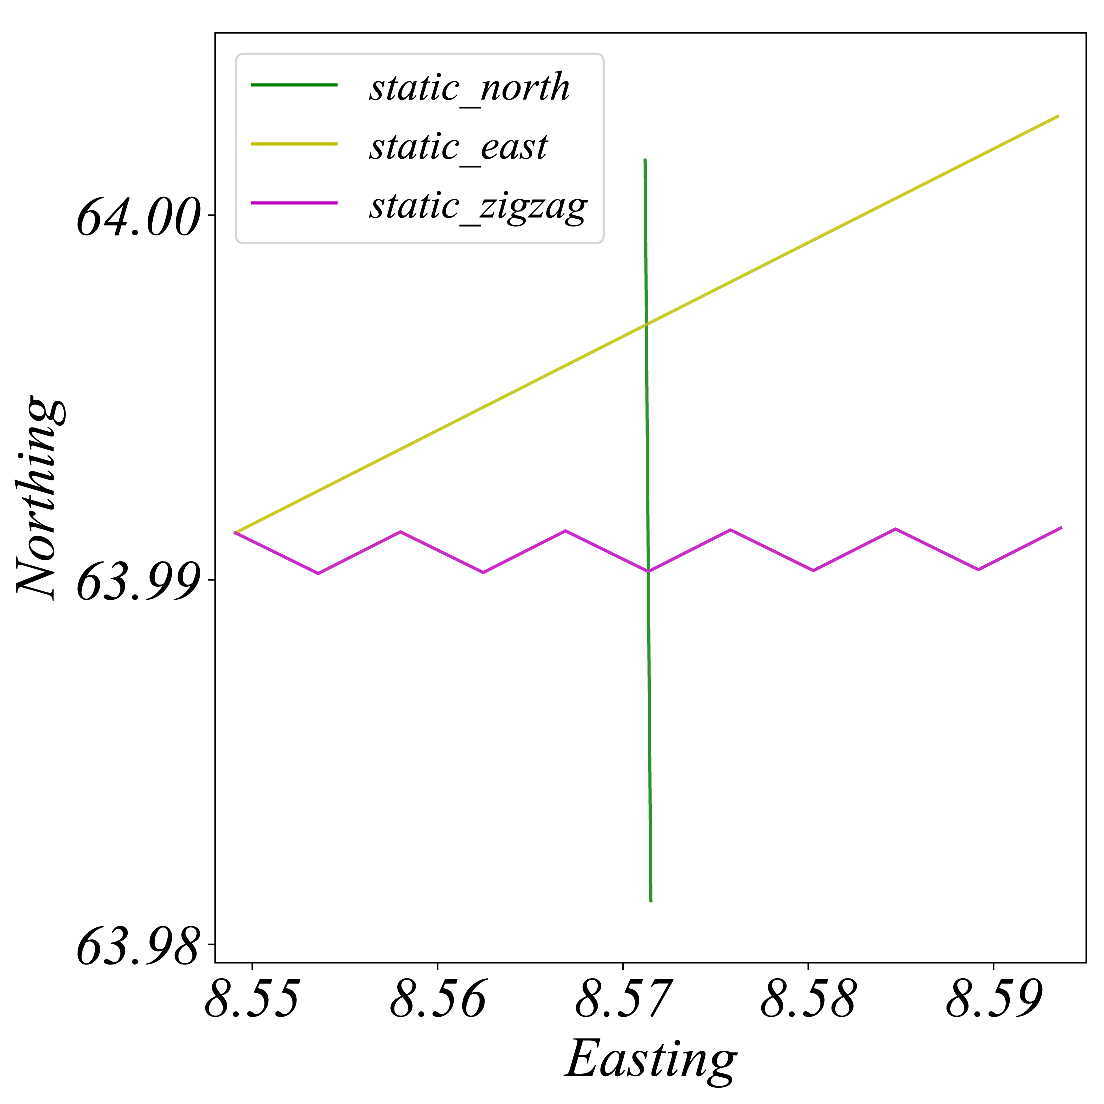
\includegraphics[height = 0.46\textwidth]{Figures/sim/route_static.pdf}\label{fig:route_static}}
  \hfill
\caption{The overlaid route choices, superimposed for the 100 replicate
  surveys with 10 sampling choices/steps.} 
\label{fig:route_choices}
\end{figure}

The naive strategy appears to get stuck in the southern part of the
domain in some cases, because it is too focused on the probabilities
near $0.5$. The myopic strategy seems to be covering a wider domain than
the look-ahead strategy, possibly because the look-ahead strategy sees
less value of going far west because it account for having to return
east again.

We further go on to study sensitivity of the result to different prior correlation values between temperature and salinity, prior standard deviations and spatial correlations, as well as those of measuring only temperature on-board the AUV (as indicated in the rows). We compare results at the end of the surveying distance. Expected ES variances are shown in Table \ref{{tab:sim_res_ev}}. Results of RMSE are in Table \ref{tab:sim_res_rmse} and explained variance in Table \ref{tab:sim_res_r2}. 
In all runs, the myopic and look-ahead strategies perform the best in terms of expected variance in the ES. Surprisingly, the myopic is on-par and even slightly better than the look-ahead strategy. Part of the reason is pruning of paths for the look-ahead strategy, but even with less pruning, the look-ahead does not outperform the myopic approach. Of course, we are able to make up cases where look-ahead beats myopic, but within our ranges of realistic input parameter values it was not easy.
The static north design is clearly better than the other two static designs. The others do not focus on the areas where the ES is really uncertain. 
By measuring temperature alone the expected variances in the ES is only slightly higher. This occurs because the ES is almost the same and because of the correlation of $0.6$ which means that temperature observations give information about salinity as well. 

For the other predictive measures, myopic and look-ahead are still doing well, clearly beating the naive approach. The static zigzag design is usually the best among the static designs for these predictive performance measures because its pattern gives more effective coverage of the domain when there is significant spatial correlation as in this case.
\begin{table}[!h]
    \centering
    \scalebox{0.87}{
    \begin{tabular}{lrrrrrr}
    \toprule
    Parameter: $E_{\by}(p[1-p])$ &  naive &  myopic &  look-ahead &  static\_north &  static\_east &  static\_zigzag \\
    \midrule
                    \rowcolor{Gray}
ts. cor. low: 0.2  &  29.65 &   27.08 &       \textbf{26.44} &         32.33 &        40.31 &          36.23 \\
ts. cor. high: 0.8 &  36.18 &   \textbf{28.42} &       30.30 &         32.99 &        37.18 &          36.04 \\
                    \rowcolor{Gray}
std. low: 0.1      &  18.26 &   15.79 &       \textbf{15.35} &         18.89 &        26.65 &          26.10 \\
std. high: 0.5     &  47.01 &   \textbf{41.31} &       43.15 &         47.92 &        52.63 &          49.71 \\
                    \rowcolor{Gray}
cor. low: 0.8      &  44.42 &   \textbf{42.02} &       42.47 &         43.84 &        46.05 &          47.82 \\
cor. high: 0.2     &  29.73 &   21.09 &       \textbf{20.43} &         27.91 &        37.60 &          34.35 \\
                    \rowcolor{Gray}
temp. only         &  38.25 &   29.16 &       \textbf{28.69} &         34.32 &        39.81 &          36.17 \\
basecase           &  35.21 &   \textbf{28.56} &       28.94 &         33.50 &        39.84 &          39.26 \\
    \bottomrule
    \end{tabular}}
    \caption{Simulation results for the final mean excursion set variance (Eq. \eqref{two_partsK}) for 20 replicates, 8 configurations, and 6 strategies.}
    \label{tab:sim_res_ev}
\end{table}

\begin{table}[!h]
    \centering
    \scalebox{0.92}{
        \begin{tabular}{lrrrrrr}
        \toprule
        Parameter: RMSE &  naive &  myopic &  look-ahead &  static\_north &  static\_east &  static\_zigzag \\
        \midrule
                \rowcolor{Gray}
ts. cor. low: 0.2  &   0.63 &    \textbf{0.57} &        0.59 &          0.62 &         0.57 &           0.59 \\
ts. cor. high: 0.8 &   0.63 &    \textbf{0.59} &        0.61 &          0.64 &         0.60 &           0.60 \\
                \rowcolor{Gray}
std. low: 0.1      &   0.39 &    0.37 &        0.38 &          0.38 &         0.40 &           \textbf{0.35} \\
std. high: 0.5     &   0.85 &    0.82 &        0.84 &          0.82 &         0.83 &           \textbf{0.81} \\  
                \rowcolor{Gray}
cor. low: 0.8      &   0.68 &    0.66 &        0.67 &          0.68 &         0.66 &           \textbf{0.65} \\
cor. high: 0.2     &   0.58 &    0.54 &        0.55 &          0.58 &         0.54 &           \textbf{0.49} \\
                \rowcolor{Gray}
temp. only         &   0.65 &    0.63 &        0.62 &          0.65 &         \textbf{0.61} &           0.62 \\
basecase           &  0.61 &   \textbf{0.56} &       \textbf{0.56} &         0.60 &        0.57 &          0.57 \\
        \bottomrule
        \end{tabular}}
    \caption{Simulation results for the final mean RMSE ($\frac{1}{B} \sum_{b=1}^{B} \sqrt{(\bmu-\tilde{\bmu})^2}$) for 20 replicates, 8 configurations, and 6 strategies.}
    \label{tab:sim_res_rmse}
\end{table}

\begin{table}[!h]
    \centering
    \scalebox{0.95}{
        \begin{tabular}{lrrrrrr}
        \toprule
        Parameter: $\bR^{2}$ &  naive &  myopic &  look-ahead &  static\_north &  static\_east &  static\_zigzag \\
        \midrule
                        \rowcolor{Gray}
ts. cor. low: 0.2  &  27.00 &   33.29 &       32.24 &         26.71 &        30.56 &          \textbf{33.50} \\
ts. cor. high: 0.8 &  23.68 &   \textbf{33.87} &       32.42 &         26.72 &        30.73 &          33.61 \\
                        \rowcolor{Gray}
std. low: 0.1      &  25.38 &   30.80 &       30.29 &         26.09 &        28.75 &          \textbf{31.66} \\
std. high: 0.5     &  26.11 &   34.22 &       32.48 &         26.95 &        31.77 &          \textbf{34.48} \\
                        \rowcolor{Gray}
cor. low: 0.8      &   8.80 &   11.50 &       11.23 &          9.56 &        12.31 &          \textbf{12.58} \\
cor. high: 0.2     &  37.57 &   \textbf{48.68} &       48.11 &         39.61 &        41.98 &          48.04 \\
                        \rowcolor{Gray}
temp. only         &  11.67 &   \textbf{22.82} &       21.98 &         18.16 &        20.77 &          22.78 \\
basecase           &  24.71 &   33.45 &       32.25 &         26.71 &        30.62 &          \textbf{33.54}\\
        \bottomrule
        \end{tabular}}
    \caption{Simulation results for the final mean explained variance ($\bR^{2}=100*(1-(\bSigma_{posterior}/\bSigma_{initial}))$) for 20 replicates, 8 configurations, and 6 strategies.}
    \label{tab:sim_res_r2}
\end{table}

\newpage

\section{Case study - Mapping a river plume}\label{sec:case_study}

To demonstrate the applicability of multivariate EP to informative oceanographic sampling, a case study mapping river plumes with an AUV is presented.
This test is done in the near Trondheim, Norway, where the Nidelva river (see Figure \ref{fig:river1}). The test focuses along the eastern shoreline due to the aforementioned Coriolis force.%, see Fig. \ref{fig:map}. 
The frontal zone therefore runs parallel to the eastern shore as indicated in pink.  enters the Trondheimsfjord. The tests were done in the late Spring of 2019, and because of snow melting in the mountains, the fresh river water is then substantially colder than the fjord water.


\subsection{Statistical model specification}

Statistical model parameters were specified based on preliminary runs. A short preliminary survey was therefore conducted upon arriving at the site, where the AUV did an initial transect to determine the environmental conditions and correlation structure.  

In these runs the trend parameters were estimated by linear regression, where both temperature and salinity are assumed to increase linearly, going west from the river mouth. Next, the residuals from the regression analysis are analyzed to study the fit of the Gaussian model and to specify the covariance parameter. 

Figure \ref{fig:parest} shows the diagnostic plots of this residual analysis. The left display show a cross-plot of temperature and salinity residuals, indicating larger variability in the salinity than in temperature, and a positive correlation ($0.5$) between the two variables. Based on the fitted bivariate Gaussian model we can compute the quadratic form of the residuals. If the Gaussian model is adequate the residuals should be approximately $\chi^2_2$ distributed. Figure \ref{fig:parest} (middle) shows the empirical cdf of these quadratic forms (solid) together with the theoretical cdf of the $\chi^2_2$ distribution. Even though there appears to be some clustering in both left and middle displays, the fit fit appears quite reasonable, and justifies the use of a Gaussian bivariate model in this case. Figure \ref{fig:parest} (right) shows the empirical variogram of the scaled residuals for temperature and salinity. The decay is similar, and seems to be negligible after about $150$ m. The resulting parameters are given in Table \ref{tab:experiment_param} below.


%Mapping the spatial extent of a frontal zones is an important problem for studying many bio-physical interactions in the ocean. The frontal zone is determined by the boundary where plumes of sediments, nutrients, and possibly pollutants spreading from the river outlet meet and interact with adjacent coastal water. Due to the lower density the plumes spread on the surface, creating a front with an sharp gradient in both temperature and salinity. 

\begin{figure}[!h] 
 \centering 
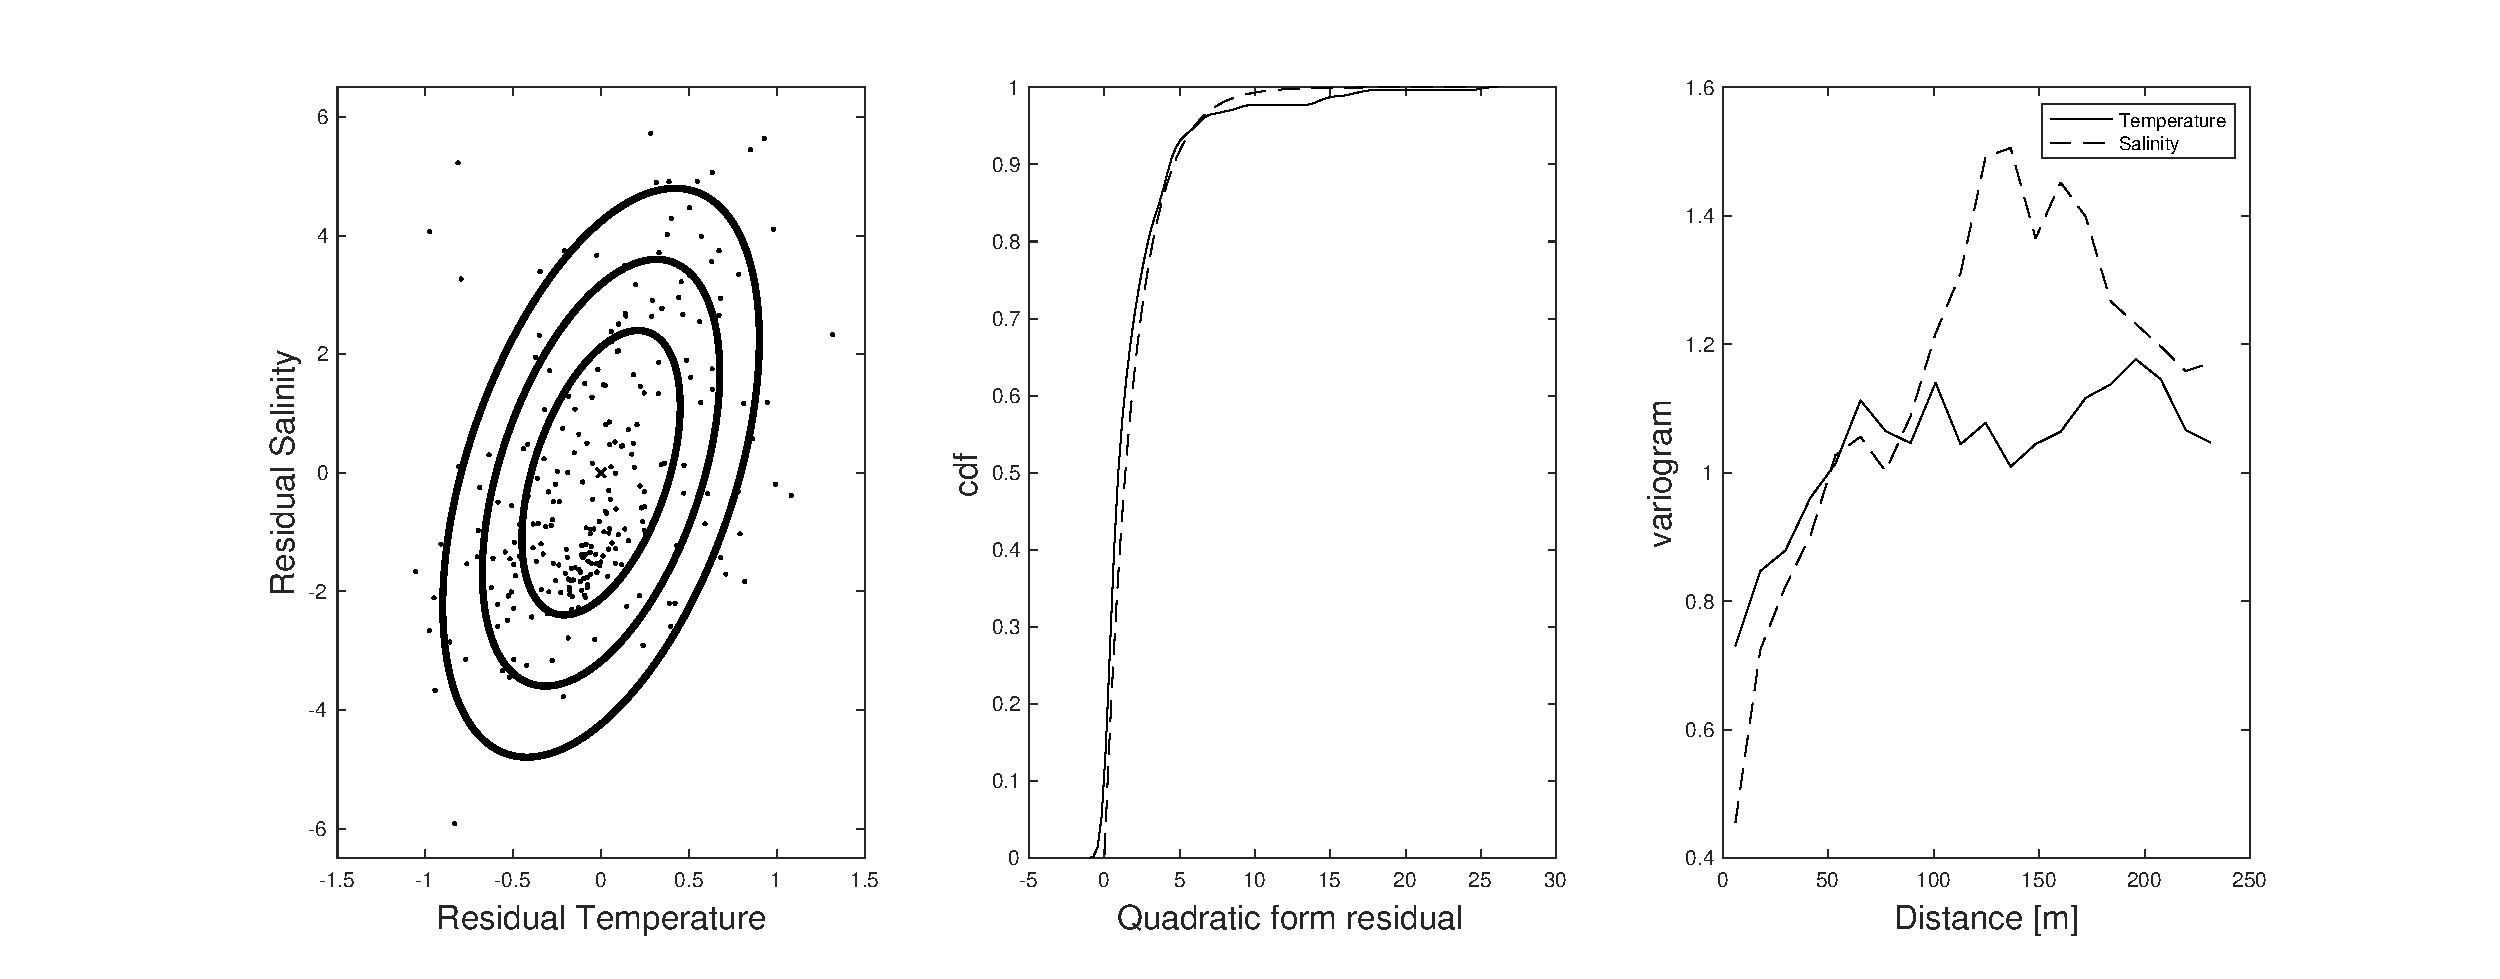
\includegraphics[width=0.98\textwidth]{Figures/field-trials/res_diag.eps}
\caption{Data analysis from a preliminary trial experiment using the AUV. Left) Residual plot of temperature and salinity along with Gaussian contours. Middle) Empirical cdf of the quadratic form of the residuals along with the theoretical cdf of the Kji-square distribution with two degrees of freedom. Right) Empirical variogram of the salinity and temperature data.} \label{fig:parest}
\end{figure}

\begin{table}[!h]
\centering
\begin{tabular}{lrr}
\toprule
Parameter & Value & Source\\
\midrule
\rowcolor{Gray}
Cross correlation temp. and sal. & 0.5 & AUV observations\\
Temp. variance &  0.20 & AUV observations (variogram)\\
\rowcolor{Gray}
Sal. variance &  5.76 & AUV observations (variogram)\\
Corr. range  & 0.15 km & AUV observations (variogram)\\
\rowcolor{Gray}
River temp. $T_{river}$ & $10.0\,^{\circ}\mathrm{C}$ & AUV observations\\
Ocean temp. $T_{ocean}$ & $11.0\,^{\circ}\mathrm{C}$ & AUV observations\\
\rowcolor{Gray}
River sal. $S_{river}$ & $14.0$g/kg & AUV observations\\
Ocean sal. $S_{ocean}$ & $22.0$g/kg & AUV observations\\
\rowcolor{Gray}
Threshold temp. & $10.5\,^{\circ}\mathrm{C}$ & $(T_{ocean}-T_{river})/2+T_{river}$\\
Threshold sal. & $22.0$g/kg & $(S_{ocean}-S_{river})/2+S_{river}$\\
\rowcolor{Gray}
\bottomrule
\end{tabular}
\caption{Model and threshold parameters found from initial AUV survey. Observations were taken across the front crossing from fresh and cold river water to saline and warmer ocean water.}
\label{tab:experiment_param}
\end{table}


These mean and covariance parameters values were then used in a field trial, where we explored the algorithm's ability to explore the front between the river and fjord water masses. 

\subsection{Experiment setup}

Two full-scale deployments were conducted with adaptive AUV sampling.
%on the 2$^{nd}$ of July 2019 spatially mapping the location of the plume from the Nidelven river (Trondheim, Norway) spreading into the Trondheimsfjord 
The AUV used the onboard autonomous agent T-REX \citep{Mcgann}, running an instance of the myopic strategy from Section \ref{sec:sampling_designs}, to control the AUV and decide between sampling locations. 

The sampling locations are distributed over an equilateral grid, as shown in Fig. \ref{fig:map} in a grey colored lattice. The robotic platform consisted of a Light AUV \citep{sousa2012lauv} equipped with a 16 Hz Seabird Fastcat-49 CTD (conductivity, temperature, and depth) sensor providing temperature and salinity measurements to the bi-variate GP model. The accuracy of the CTD instrument is $\pm 0.0003$ S/m (conductivity) and $\pm0.002\,^{\circ}\mathrm{C}$ (temperature).

%\begin{figure}[!h] 
%\centering 
%
\includegraphics[width=0.98\textwidth]{Figures/harald.jpg}
%\caption{The light AUV platform (Harald) for upper water-
%column exploration used in the experiment.}
%\label{fig:harald_auv}
%\end{figure} 


The sampling strategy is designed around sequentially visiting waypoints, where arrival at a desired waypoint subsequently triggers the myopic strategy to evaluate and find the next waypoint based on the ES variance formulated in Eq. \eqref{critSEQ}. The waypoint --and associated sampling-- that results in lowering the ES variance the most is selected. For the field trials, the AUV started in the lower middle of the graph with a GP prior estimate of the environment given as a linear gradient from west to east, between the initially measured temperature and salinity. Each AUV survey/mission was set to take approx. 40 min, visiting 15 waypoints on the grid, with the AUV running at the surface to better capture the plume. The GP model assimilated temperature and salinity data continuously with an update frequency of 30 sec.

\subsection{Results}

Two missions, Survey 1 and 2, was run successively from 11:00 AM to 01:00 PM, with a short break in between. The resulting path between the selected waypoints are shown in spatial context in Fig. \ref{fig:map}, both within the expected frontal region. The recorded temperatures are shown as colored trails in Fig. \ref{fig:res_both}, clearly showing the temperature difference between ocean and river waters. The temperatures are then shown separately overlaid with the estimated ES for each survey in Fig. \ref{fig:res1} and \ref{fig:res2}. 

Both Survey 1 and 2, successfully estimates and navigates the separation zone crossing the front multiple times. As conditions change between the two deployments the resulting path (after waypoint 5) deviate. Survey 1 continue northwards tracking the north-eastern part of the front, while Survey 2 turns west mapping the south-western part. The final prediction of the front location given Fig. \ref{fig:res3} and \ref{fig:res4}, correspond with one another yielding a picture of the front gradually bending off towards north east. The amount of exploration done by Survey 1 is greater than Survey 2, coming close to the survey area boarders in the south-western corner. A longer planning horizon would identify and discourage such choices. 

\begin{figure}[!h]
\centering
\subfigure[Survey map.]{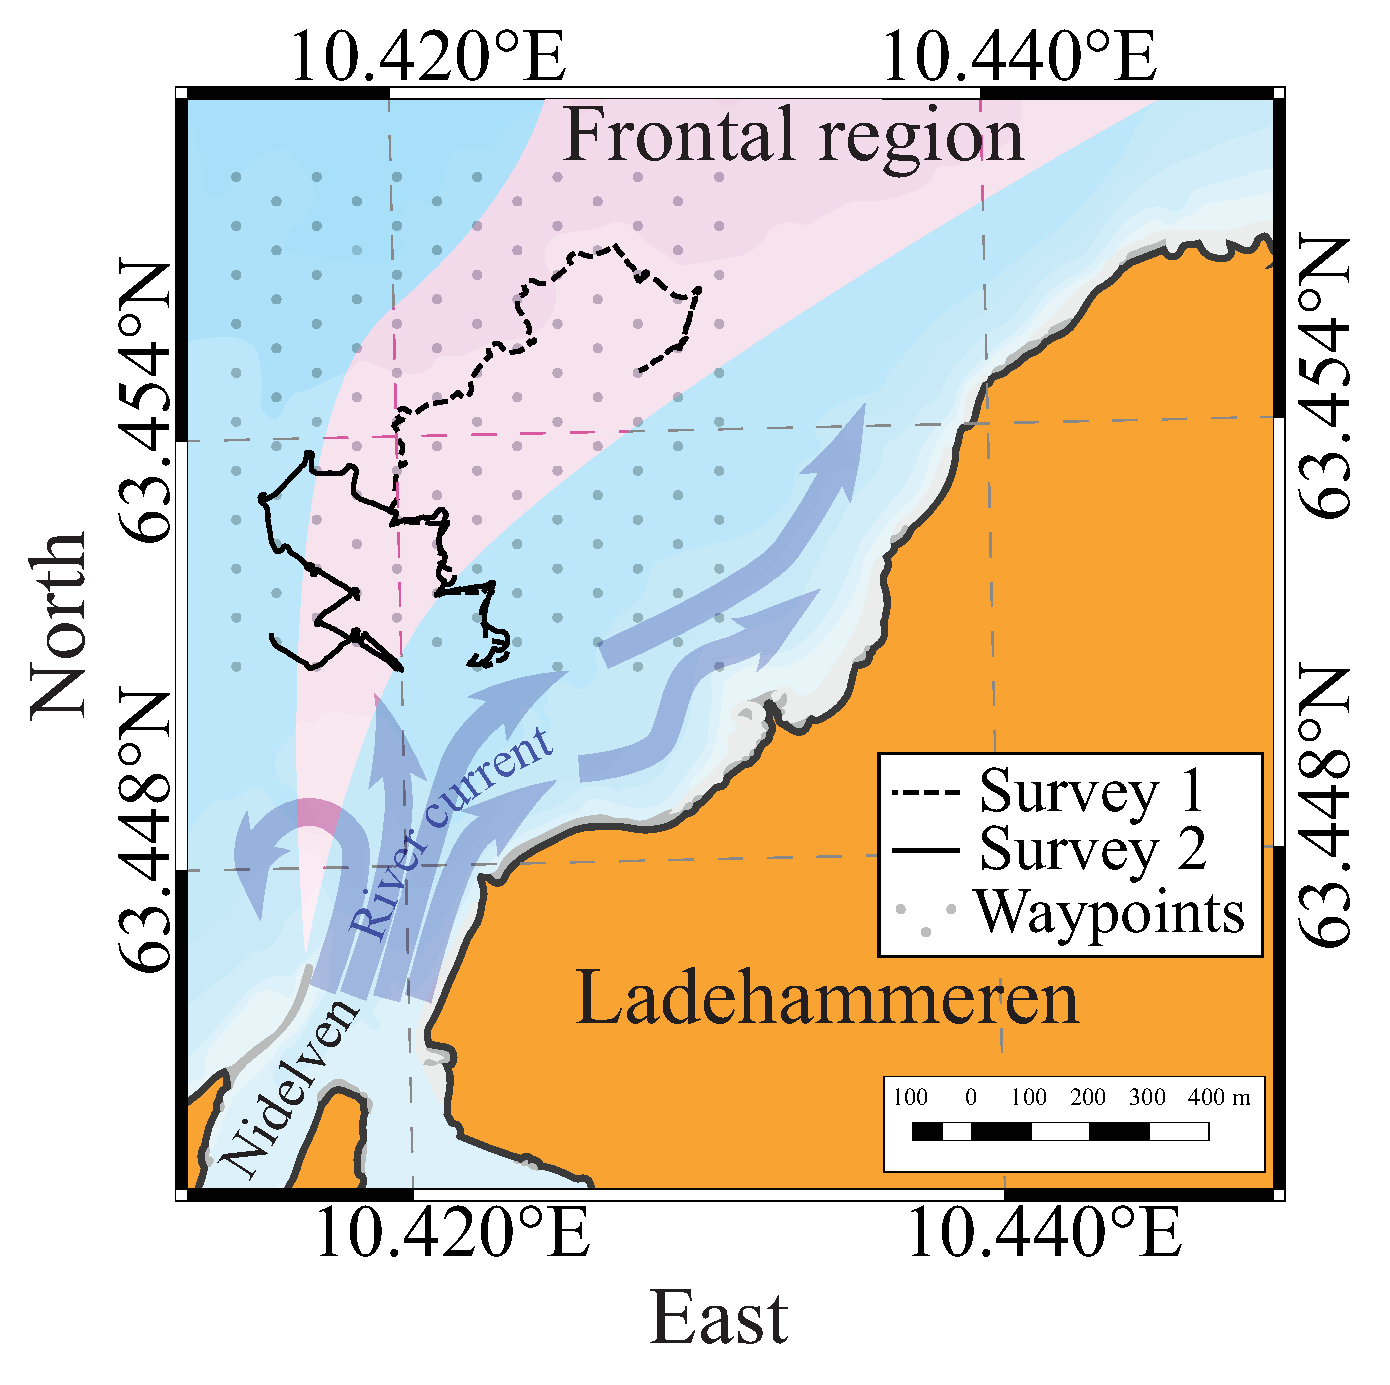
\includegraphics[height = 0.31\textwidth]{Figures/field-trials/alt_map.eps}\label{fig:map}}
\hfill
\subfigure[Temperature tracks.]{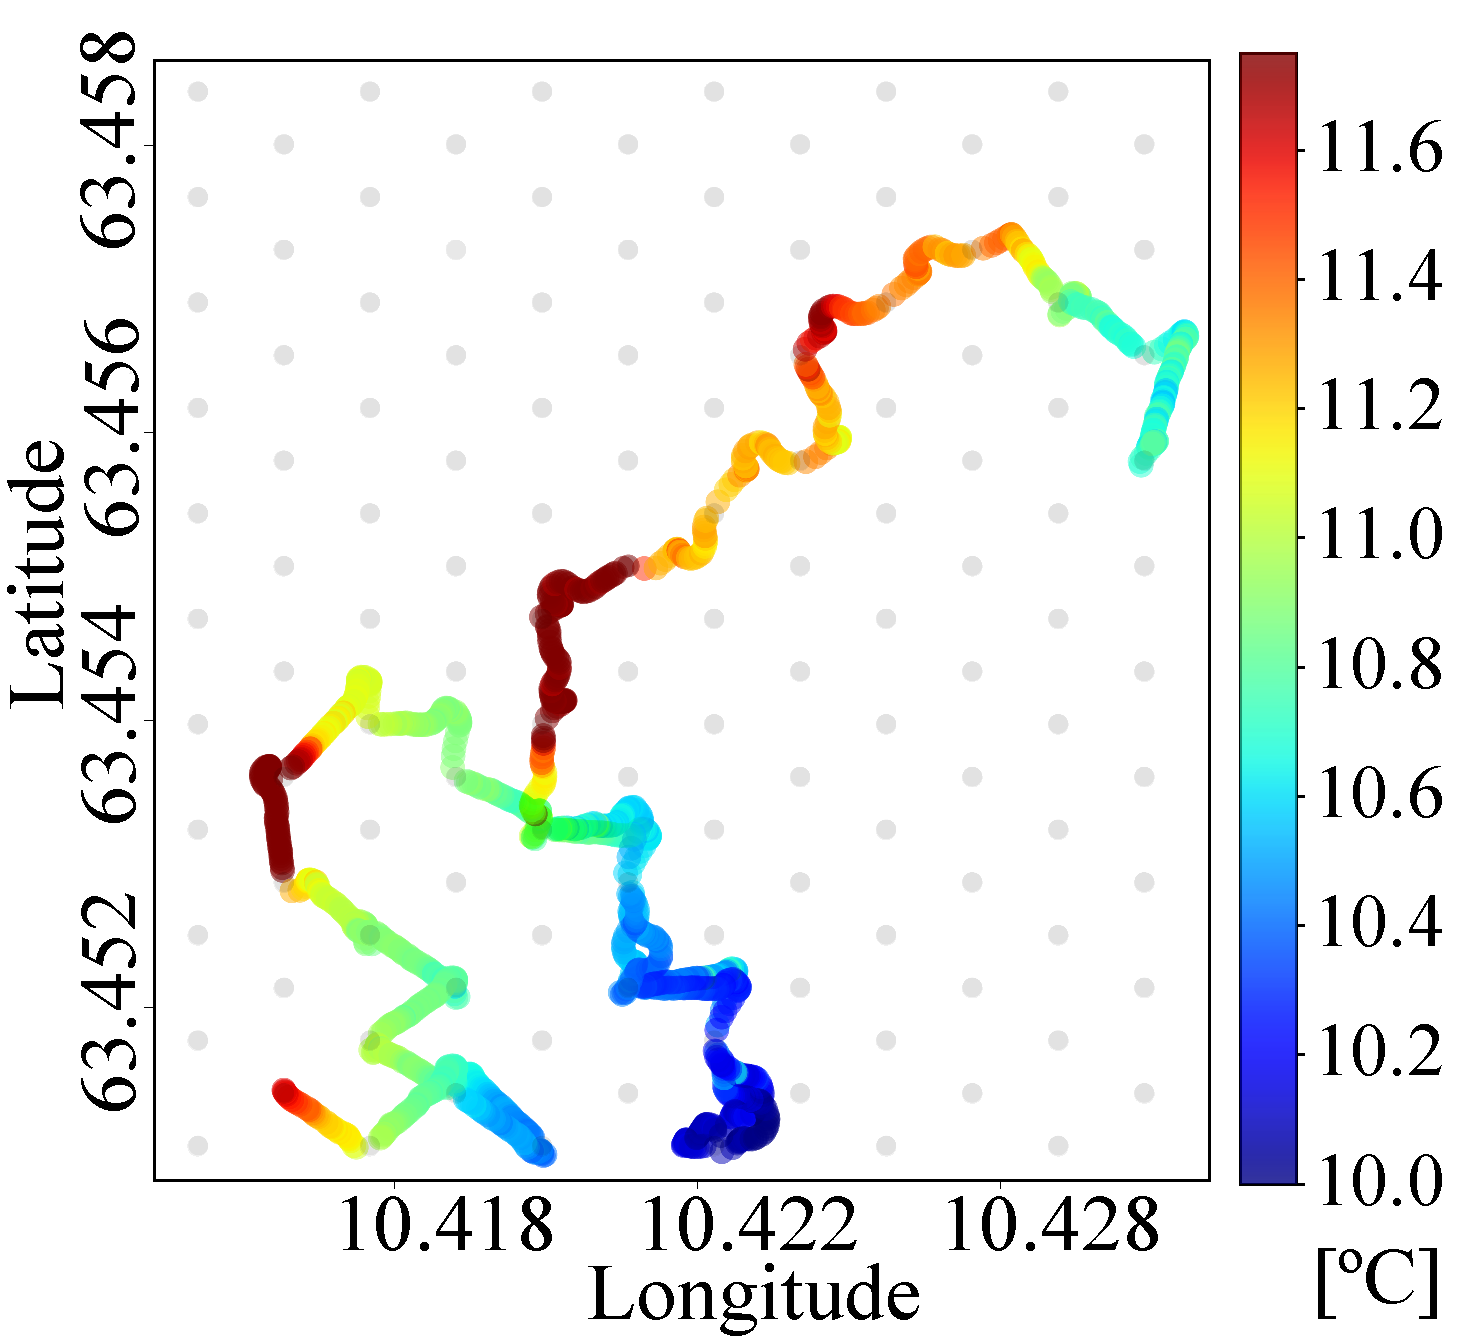
\includegraphics[height = 0.31\textwidth]{Figures/field-trials/auv.pdf}\label{fig:res_both}}
\hfill
\subfigure[Survey 1]{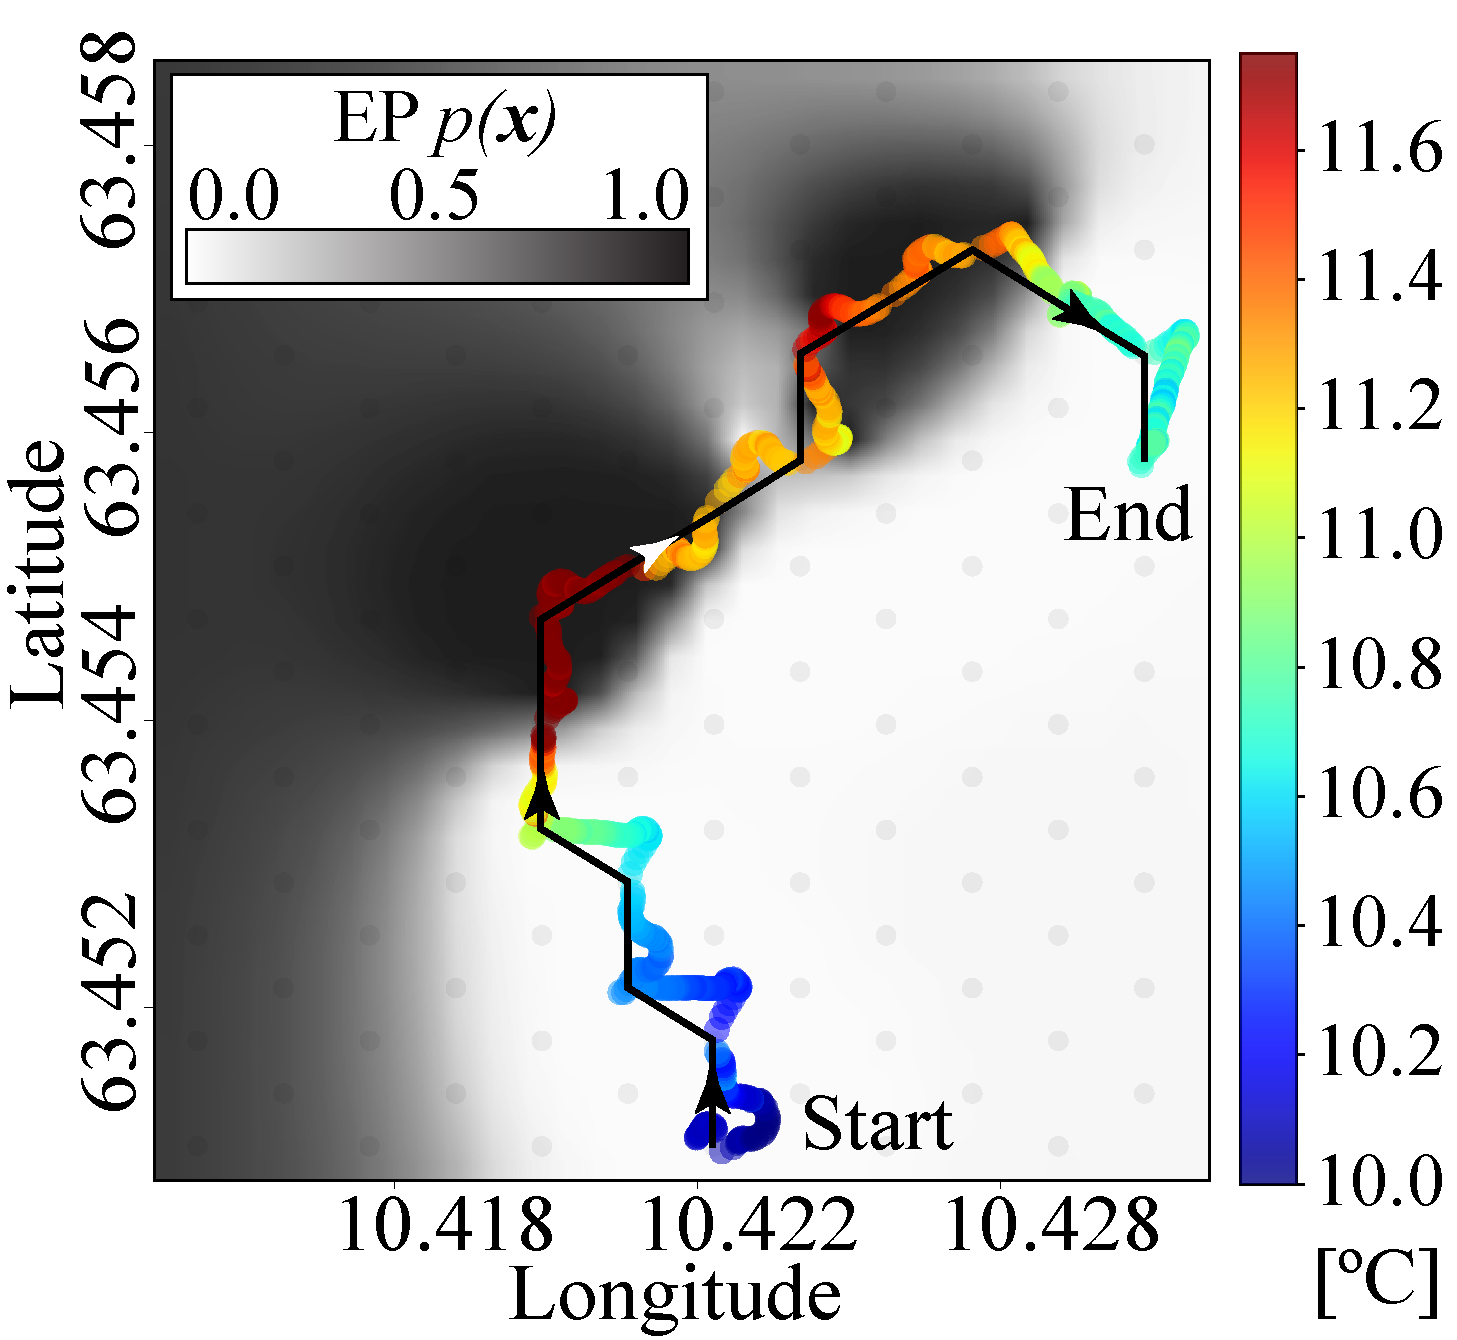
\includegraphics[height = 0.31\textwidth]{Figures/field-trials/auv1_es.pdf}\label{fig:res1}}
\hfill
\subfigure[Survey 2]{\includegraphics[height = 0.31\textwidth]{Figures/field-trials/auv4_es.pdf}\label{fig:res2}}
\hfill
\subfigure[ES for Survey 1.]{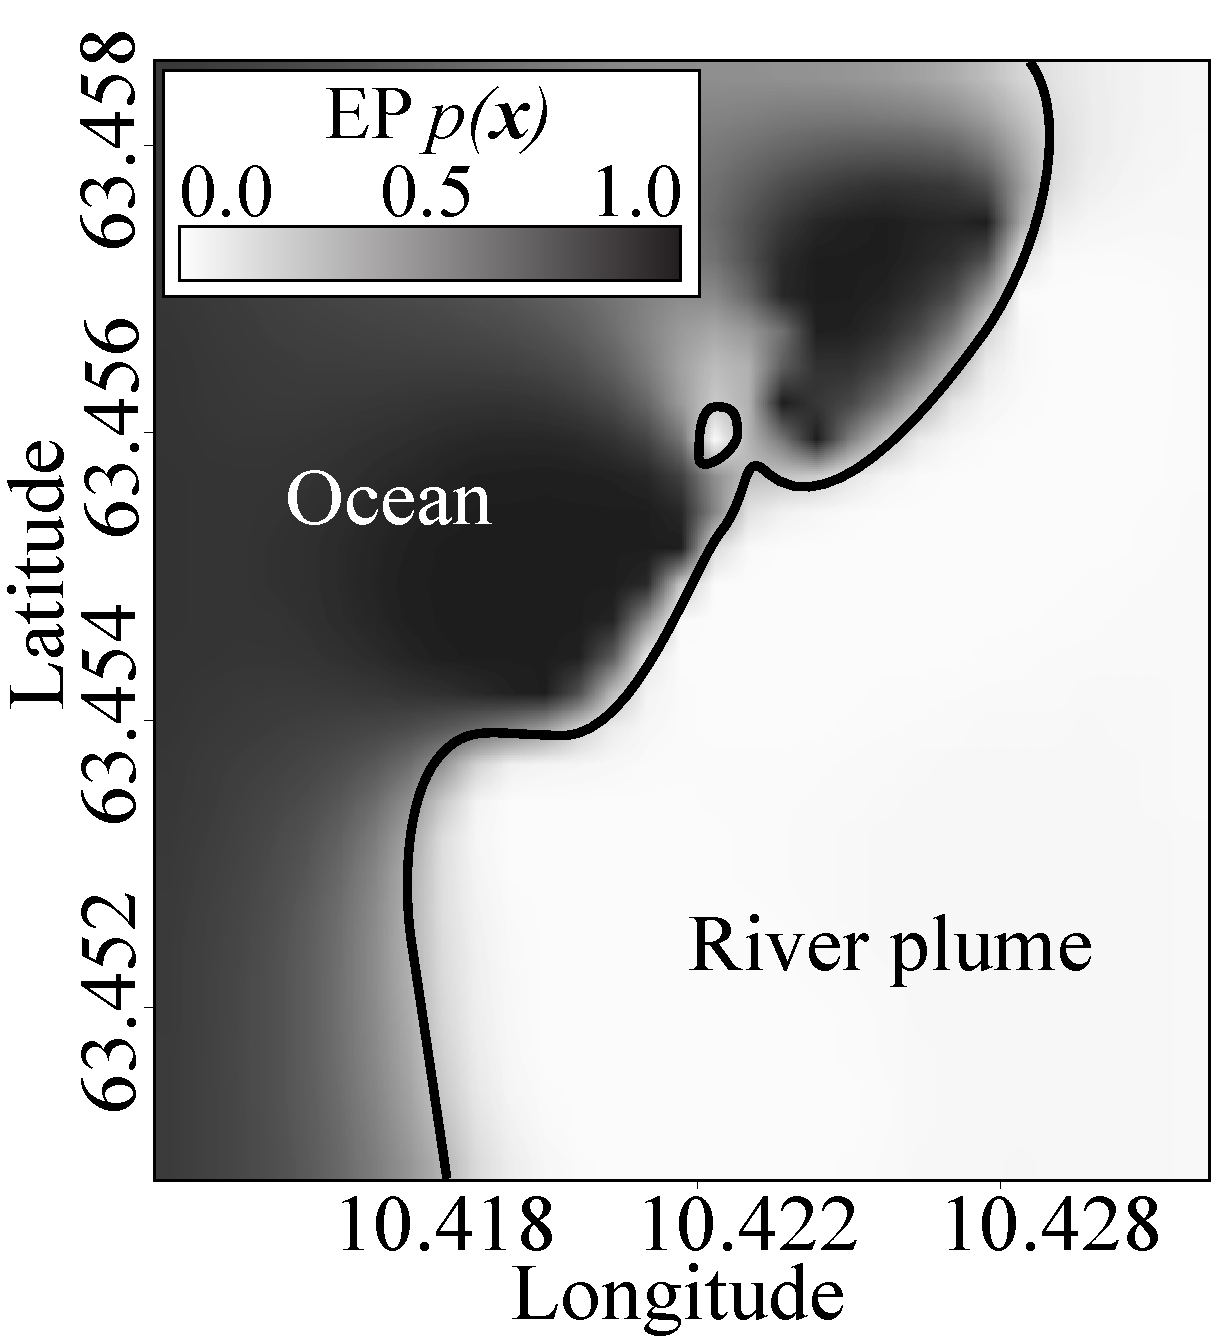
\includegraphics[height = 0.31\textwidth]{Figures/field-trials/ep_1.pdf}\label{fig:res3}}
\hfill
\subfigure[ES for Survey 2.]{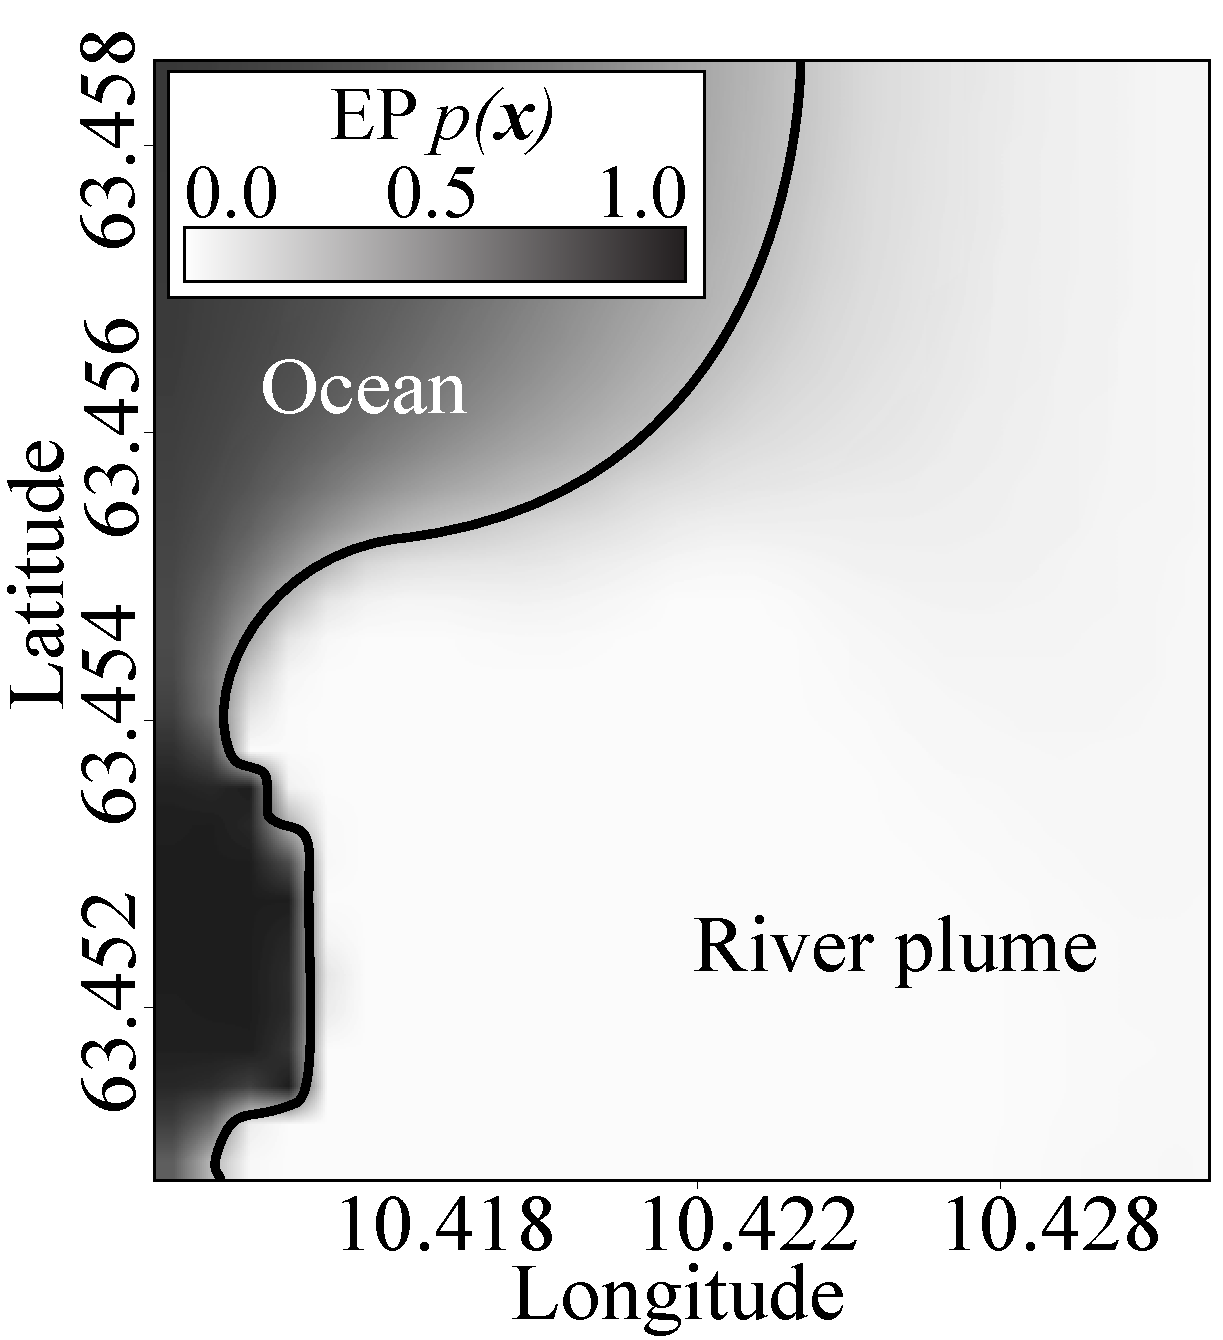
\includegraphics[height = 0.31\textwidth]{Figures/field-trials/ep_4.pdf}\label{fig:res4}}
\caption{Results from mapping the Nidelven river} 
\label{fig:results}
\end{figure}


%\begin{figure}[!h] 
% \centering 
%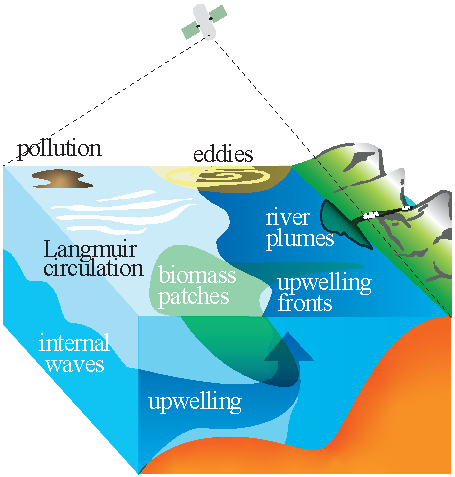
\includegraphics[width=0.48\textwidth]{Figures/envir_ocean.pdf}
%\caption{Ocean observation is moving away from %single-ship sampling
%towards more collaborative networked operations in %order to resolve
%the numerous processes and their interaction.} %\label{fig:envir}
%\end{figure}


\section{Closing remarks}\label{sec:concl_disc}

The methods presented in this paper are shown to be useful in characterizing the frontal water masses where cold river water is separated from the warmer saltwater. The study did not consider any temporal effects, which would surely be relevant on a longer time scale. We consider the extension to spatio-temporal modeling future work, and we envision that advection-diffusion equations could be useful in this kind of modeling \cite{sigrist2015stochastic}. 
For more complicated oceanographic phenomena, we the methods must maybe be extended to non-Gaussian phenomena and with more complex dynamical models. 

Regarding the autonomous sampling, more effort can be spent on approximating the look-ahead steps, but it is perhaps more interesting to explore the additional flexibility that can be gained by having two or more AUVs exploring a spatial or spatio-temporal domain together. It might then be useful to sample different parts of the space, and maybe move in parallel to best capture the excursion set. 

\section*{Acknowledgements}
Thanks to SINTEF Ocean, AMOS, etc..

%\begin{supplement}
%\sname{Supplement A}\label{suppA}
%\stitle{Title of the Supplement A}
%\slink[url]{http://www.e-publications.org/ims/support/dowload/imsart-ims.zip}
%\sdescription{Dum esset rex in
%accubitu suo, nardus mea dedit odorem suavitatis. Quoniam confortavit
%seras portarum tuarum, benedixit filiis tuis in te. Qui posuit fines tuos}
%\end{supplement}

% == Adding references
\footnotesize
\bibliographystyle{apalike}
\bibliography{ref}


% AOS,AOAS: If there are supplements please fill:
%\begin{supplement}[id=suppA]
%  \sname{Supplement A}
%  \stitle{Title}
%  \slink[doi]{10.1214/00-AOASXXXXSUPP}
%  \sdatatype{.pdf}" 
%  \sdescription{Some text}
%\end{supplement}


\end{document}

%\begin{enumerate}
%\item  This is the first item of an enumerated list.  Each item
%      in the list is marked with a ``tick.''  The document
%      style determines what kind of tick mark is used.
%\item  This is the second item of the list.  It contains another
%      list nested inside it.  The three inner lists are an {\em enumerated}
%      list.
%    \begin{enumerate}
%       \item This is the first item of an enumerated list that
%            is nested within the enumerated list.
%          \item This is the second item of the inner list.  \LaTeX\
%            allows you to nest lists deeper than you really should.
%      \end{enumerate}
%      This is the rest of the second item of the outer list.  It
%      is no more interesting than any other part of the item.
%   \item  This is the third item of the list.
%\end{enumerate}